\documentclass[twoside]{book}

% Packages required by doxygen
\usepackage{calc}
\usepackage{doxygen}
\usepackage{graphicx}
\usepackage[utf8]{inputenc}
\usepackage{makeidx}
\usepackage{multicol}
\usepackage{multirow}
\usepackage{textcomp}
\usepackage[table]{xcolor}

% Font selection
\usepackage[T1]{fontenc}
\usepackage{mathptmx}
\usepackage[scaled=.90]{helvet}
\usepackage{courier}
\usepackage{amssymb}
\usepackage{sectsty}
\renewcommand{\familydefault}{\sfdefault}
\allsectionsfont{%
  \fontseries{bc}\selectfont%
  \color{darkgray}%
}
\renewcommand{\DoxyLabelFont}{%
  \fontseries{bc}\selectfont%
  \color{darkgray}%
}

% Page & text layout
\usepackage{geometry}
\geometry{%
  a4paper,%
  top=2.5cm,%
  bottom=2.5cm,%
  left=2.5cm,%
  right=2.5cm%
}
\tolerance=750
\hfuzz=15pt
\hbadness=750
\setlength{\emergencystretch}{15pt}
\setlength{\parindent}{0cm}
\setlength{\parskip}{0.2cm}
\makeatletter
\renewcommand{\paragraph}{%
  \@startsection{paragraph}{4}{0ex}{-1.0ex}{1.0ex}{%
    \normalfont\normalsize\bfseries\SS@parafont%
  }%
}
\renewcommand{\subparagraph}{%
  \@startsection{subparagraph}{5}{0ex}{-1.0ex}{1.0ex}{%
    \normalfont\normalsize\bfseries\SS@subparafont%
  }%
}
\makeatother

% Headers & footers
\usepackage{fancyhdr}
\pagestyle{fancyplain}
\fancyhead[LE]{\fancyplain{}{\bfseries\thepage}}
\fancyhead[CE]{\fancyplain{}{}}
\fancyhead[RE]{\fancyplain{}{\bfseries\leftmark}}
\fancyhead[LO]{\fancyplain{}{\bfseries\rightmark}}
\fancyhead[CO]{\fancyplain{}{}}
\fancyhead[RO]{\fancyplain{}{\bfseries\thepage}}
\fancyfoot[LE]{\fancyplain{}{}}
\fancyfoot[CE]{\fancyplain{}{}}
\fancyfoot[RE]{\fancyplain{}{\bfseries\scriptsize Generated on Sat Aug 31 2013 19\-:31\-:56 for Magistarski aplikacija by Doxygen }}
\fancyfoot[LO]{\fancyplain{}{\bfseries\scriptsize Generated on Sat Aug 31 2013 19\-:31\-:56 for Magistarski aplikacija by Doxygen }}
\fancyfoot[CO]{\fancyplain{}{}}
\fancyfoot[RO]{\fancyplain{}{}}
\renewcommand{\footrulewidth}{0.4pt}
\renewcommand{\chaptermark}[1]{%
  \markboth{#1}{}%
}
\renewcommand{\sectionmark}[1]{%
  \markright{\thesection\ #1}%
}

% Indices & bibliography
\usepackage{natbib}
\usepackage[titles]{tocloft}
\setcounter{tocdepth}{3}
\setcounter{secnumdepth}{5}
\makeindex

% Hyperlinks (required, but should be loaded last)
\usepackage{ifpdf}
\ifpdf
  \usepackage[pdftex,pagebackref=true]{hyperref}
\else
  \usepackage[ps2pdf,pagebackref=true]{hyperref}
\fi
\hypersetup{%
  colorlinks=true,%
  linkcolor=blue,%
  citecolor=blue,%
  unicode%
}

% Custom commands
\newcommand{\clearemptydoublepage}{%
  \newpage{\pagestyle{empty}\cleardoublepage}%
}


%===== C O N T E N T S =====

\begin{document}

% Titlepage & ToC
\hypersetup{pageanchor=false}
\pagenumbering{roman}
\begin{titlepage}
\vspace*{7cm}
\begin{center}%
{\Large Magistarski aplikacija \\[1ex]\large 1 }\\
\vspace*{1cm}
{\large Generated by Doxygen 1.8.5}\\
\vspace*{0.5cm}
{\small Sat Aug 31 2013 19:31:56}\\
\end{center}
\end{titlepage}
\clearemptydoublepage
\tableofcontents
\clearemptydoublepage
\pagenumbering{arabic}
\hypersetup{pageanchor=true}

%--- Begin generated contents ---
\chapter{Hierarchical Index}
\section{Class Hierarchy}
This inheritance list is sorted roughly, but not completely, alphabetically\-:\begin{DoxyCompactList}
\item \contentsline{section}{Duz}{\pageref{struct_duz}}{}
\item \contentsline{section}{Elementarni\-Interval}{\pageref{struct_elementarni_interval}}{}
\item \contentsline{section}{Krajnja\-Tacka\-Duzi}{\pageref{struct_krajnja_tacka_duzi}}{}
\item \contentsline{section}{Poredjenje\-Po\-X}{\pageref{struct_poredjenje_po_x}}{}
\item \contentsline{section}{Poredjenje\-Po\-Y}{\pageref{struct_poredjenje_po_y}}{}
\item Q\-Widget\begin{DoxyCompactList}
\item \contentsline{section}{Pretraga\-Prostora}{\pageref{class_pretraga_prostora}}{}
\end{DoxyCompactList}
\item \contentsline{section}{Stablo\-Duzi}{\pageref{class_stablo_duzi}}{}
\item \contentsline{section}{Stablo\-Raspona}{\pageref{class_stablo_raspona}}{}
\end{DoxyCompactList}

\chapter{Class Index}
\section{Class List}
Here are the classes, structs, unions and interfaces with brief descriptions\-:\begin{DoxyCompactList}
\item\contentsline{section}{\hyperlink{struct_duz}{Duz} }{\pageref{struct_duz}}{}
\item\contentsline{section}{\hyperlink{struct_elementarni_interval}{Elementarni\-Interval} }{\pageref{struct_elementarni_interval}}{}
\item\contentsline{section}{\hyperlink{struct_krajnja_tacka_duzi}{Krajnja\-Tacka\-Duzi} }{\pageref{struct_krajnja_tacka_duzi}}{}
\item\contentsline{section}{\hyperlink{struct_poredjenje_po_x}{Poredjenje\-Po\-X} }{\pageref{struct_poredjenje_po_x}}{}
\item\contentsline{section}{\hyperlink{struct_poredjenje_po_y}{Poredjenje\-Po\-Y} }{\pageref{struct_poredjenje_po_y}}{}
\item\contentsline{section}{\hyperlink{class_pretraga_prostora}{Pretraga\-Prostora} }{\pageref{class_pretraga_prostora}}{}
\item\contentsline{section}{\hyperlink{class_stablo_duzi}{Stablo\-Duzi} }{\pageref{class_stablo_duzi}}{}
\item\contentsline{section}{\hyperlink{class_stablo_raspona}{Stablo\-Raspona} }{\pageref{class_stablo_raspona}}{}
\end{DoxyCompactList}

\chapter{File Index}
\section{File List}
Here is a list of all files with brief descriptions\-:\begin{DoxyCompactList}
\item\contentsline{section}{\hyperlink{main_8cpp}{main.\-cpp} }{\pageref{main_8cpp}}{}
\item\contentsline{section}{\hyperlink{pretraga__raspona_8cpp}{pretraga\-\_\-raspona.\-cpp} }{\pageref{pretraga__raspona_8cpp}}{}
\item\contentsline{section}{\hyperlink{pretraga__raspona_8h}{pretraga\-\_\-raspona.\-h} }{\pageref{pretraga__raspona_8h}}{}
\item\contentsline{section}{\hyperlink{resource_8h}{resource.\-h} }{\pageref{resource_8h}}{}
\item\contentsline{section}{\hyperlink{stablo__duzi_8cpp}{stablo\-\_\-duzi.\-cpp} }{\pageref{stablo__duzi_8cpp}}{}
\item\contentsline{section}{\hyperlink{stablo__duzi_8h}{stablo\-\_\-duzi.\-h} }{\pageref{stablo__duzi_8h}}{}
\item\contentsline{section}{\hyperlink{stablo__raspona_8cpp}{stablo\-\_\-raspona.\-cpp} }{\pageref{stablo__raspona_8cpp}}{}
\item\contentsline{section}{\hyperlink{stablo__raspona_8h}{stablo\-\_\-raspona.\-h} }{\pageref{stablo__raspona_8h}}{}
\item\contentsline{section}{\hyperlink{strukture_8h}{strukture.\-h} }{\pageref{strukture_8h}}{}
\item\contentsline{section}{backup/\hyperlink{backup_2stablo__raspona_8cpp}{stablo\-\_\-raspona.\-cpp} }{\pageref{backup_2stablo__raspona_8cpp}}{}
\item\contentsline{section}{backup/\hyperlink{backup_2stablo__raspona_8h}{stablo\-\_\-raspona.\-h} }{\pageref{backup_2stablo__raspona_8h}}{}
\item\contentsline{section}{backup/\hyperlink{backup_2strukture_8h}{strukture.\-h} }{\pageref{backup_2strukture_8h}}{}
\item\contentsline{section}{Generated\-Files/\hyperlink{qrc__resursi_8cpp}{qrc\-\_\-resursi.\-cpp} }{\pageref{qrc__resursi_8cpp}}{}
\item\contentsline{section}{Generated\-Files/\-Debug/\hyperlink{_debug_2moc__pretraga__raspona_8cpp}{moc\-\_\-pretraga\-\_\-raspona.\-cpp} }{\pageref{_debug_2moc__pretraga__raspona_8cpp}}{}
\item\contentsline{section}{Generated\-Files/\-Release/\hyperlink{_release_2moc__pretraga__raspona_8cpp}{moc\-\_\-pretraga\-\_\-raspona.\-cpp} }{\pageref{_release_2moc__pretraga__raspona_8cpp}}{}
\end{DoxyCompactList}

\chapter{Class Documentation}
\hypertarget{struct_duz}{\section{Duz Struct Reference}
\label{struct_duz}\index{Duz@{Duz}}
}


{\ttfamily \#include $<$strukture.\-h$>$}

\subsection*{Public Member Functions}
\begin{DoxyCompactItemize}
\item 
int \hyperlink{struct_duz_a554fe11a180cd764811139fd01bf4497}{vrati\-Id\-Duzi} ()
\item 
void \hyperlink{struct_duz_abd5a20344f28f0aa7e1866158eee381e}{postavi\-I\-D\-Duzi} (int id\-Duzi)
\item 
bool \hyperlink{struct_duz_aeefdf37bfc9720b43463bf8bc938e9ec}{jel\-Oznacena} ()
\item 
void \hyperlink{struct_duz_a387f037e652d79a998985a2f9893614a}{oznaci\-Duz} ()
\item 
void \hyperlink{struct_duz_a0c9418b7bb2ae6da48f29622371738ba}{ponisti\-Oznacenu\-Duz} ()
\item 
int \hyperlink{struct_duz_a2662b456f15f42794ddb5c1bfc3f6bb4}{vrati\-Pocetnu\-Koordinatu} (int d)
\item 
Q\-Point \hyperlink{struct_duz_a3110e0ae026af8d6bb2d5de7662e7f8b}{vrati\-Pocetnu\-Koordinatu} ()
\item 
Q\-Point \hyperlink{struct_duz_af397176a5357fecb7f785ad9685d53b2}{vrati\-Krajnju\-Koordinatu} ()
\item 
int \hyperlink{struct_duz_a3729d02c0b3d5b8181b398dc81ec79a4}{vrati\-Krajnju\-Koordinatu} (int d)
\item 
void \hyperlink{struct_duz_a792b22a53508d3c3414bd6eba4903bb3}{postavi\-Pocetnu\-Koordinatu} (Q\-Point pocetna\-Koord)
\item 
void \hyperlink{struct_duz_a6d90841b83d7f5fe8cdd1c5f53b97396}{postavi\-Krajnju\-Koordinatu} (Q\-Point krajnja\-Koord)
\item 
int \hyperlink{struct_duz_a554fe11a180cd764811139fd01bf4497}{vrati\-Id\-Duzi} ()
\begin{DoxyCompactList}\small\item\em Identifikacija duzi. \end{DoxyCompactList}\item 
void \hyperlink{struct_duz_abd5a20344f28f0aa7e1866158eee381e}{postavi\-I\-D\-Duzi} (int id\-Duzi)
\item 
bool \hyperlink{struct_duz_aeefdf37bfc9720b43463bf8bc938e9ec}{jel\-Oznacena} ()
\item 
void \hyperlink{struct_duz_a387f037e652d79a998985a2f9893614a}{oznaci\-Duz} ()
\item 
void \hyperlink{struct_duz_a0c9418b7bb2ae6da48f29622371738ba}{ponisti\-Oznacenu\-Duz} ()
\item 
int \hyperlink{struct_duz_a2662b456f15f42794ddb5c1bfc3f6bb4}{vrati\-Pocetnu\-Koordinatu} (int d)
\item 
Q\-Point \hyperlink{struct_duz_a3110e0ae026af8d6bb2d5de7662e7f8b}{vrati\-Pocetnu\-Koordinatu} ()
\item 
Q\-Point \hyperlink{struct_duz_af397176a5357fecb7f785ad9685d53b2}{vrati\-Krajnju\-Koordinatu} ()
\item 
int \hyperlink{struct_duz_a3729d02c0b3d5b8181b398dc81ec79a4}{vrati\-Krajnju\-Koordinatu} (int d)
\item 
void \hyperlink{struct_duz_a792b22a53508d3c3414bd6eba4903bb3}{postavi\-Pocetnu\-Koordinatu} (Q\-Point pocetna\-Koord)
\item 
void \hyperlink{struct_duz_a6d90841b83d7f5fe8cdd1c5f53b97396}{postavi\-Krajnju\-Koordinatu} (Q\-Point krajnja\-Koord)
\end{DoxyCompactItemize}


\subsection{Detailed Description}


Definition at line 9 of file strukture.\-h.



\subsection{Member Function Documentation}
\hypertarget{struct_duz_aeefdf37bfc9720b43463bf8bc938e9ec}{\index{Duz@{Duz}!jel\-Oznacena@{jel\-Oznacena}}
\index{jel\-Oznacena@{jel\-Oznacena}!Duz@{Duz}}
\subsubsection[{jel\-Oznacena}]{\setlength{\rightskip}{0pt plus 5cm}bool Duz\-::jel\-Oznacena (
\begin{DoxyParamCaption}
{}
\end{DoxyParamCaption}
)\hspace{0.3cm}{\ttfamily [inline]}}}\label{struct_duz_aeefdf37bfc9720b43463bf8bc938e9ec}


Definition at line 23 of file strukture.\-h.

\hypertarget{struct_duz_aeefdf37bfc9720b43463bf8bc938e9ec}{\index{Duz@{Duz}!jel\-Oznacena@{jel\-Oznacena}}
\index{jel\-Oznacena@{jel\-Oznacena}!Duz@{Duz}}
\subsubsection[{jel\-Oznacena}]{\setlength{\rightskip}{0pt plus 5cm}bool Duz\-::jel\-Oznacena (
\begin{DoxyParamCaption}
{}
\end{DoxyParamCaption}
)\hspace{0.3cm}{\ttfamily [inline]}}}\label{struct_duz_aeefdf37bfc9720b43463bf8bc938e9ec}


Definition at line 24 of file strukture.\-h.

\hypertarget{struct_duz_a387f037e652d79a998985a2f9893614a}{\index{Duz@{Duz}!oznaci\-Duz@{oznaci\-Duz}}
\index{oznaci\-Duz@{oznaci\-Duz}!Duz@{Duz}}
\subsubsection[{oznaci\-Duz}]{\setlength{\rightskip}{0pt plus 5cm}void Duz\-::oznaci\-Duz (
\begin{DoxyParamCaption}
{}
\end{DoxyParamCaption}
)\hspace{0.3cm}{\ttfamily [inline]}}}\label{struct_duz_a387f037e652d79a998985a2f9893614a}


Definition at line 26 of file strukture.\-h.

\hypertarget{struct_duz_a387f037e652d79a998985a2f9893614a}{\index{Duz@{Duz}!oznaci\-Duz@{oznaci\-Duz}}
\index{oznaci\-Duz@{oznaci\-Duz}!Duz@{Duz}}
\subsubsection[{oznaci\-Duz}]{\setlength{\rightskip}{0pt plus 5cm}void Duz\-::oznaci\-Duz (
\begin{DoxyParamCaption}
{}
\end{DoxyParamCaption}
)\hspace{0.3cm}{\ttfamily [inline]}}}\label{struct_duz_a387f037e652d79a998985a2f9893614a}


Definition at line 27 of file strukture.\-h.

\hypertarget{struct_duz_a0c9418b7bb2ae6da48f29622371738ba}{\index{Duz@{Duz}!ponisti\-Oznacenu\-Duz@{ponisti\-Oznacenu\-Duz}}
\index{ponisti\-Oznacenu\-Duz@{ponisti\-Oznacenu\-Duz}!Duz@{Duz}}
\subsubsection[{ponisti\-Oznacenu\-Duz}]{\setlength{\rightskip}{0pt plus 5cm}void Duz\-::ponisti\-Oznacenu\-Duz (
\begin{DoxyParamCaption}
{}
\end{DoxyParamCaption}
)\hspace{0.3cm}{\ttfamily [inline]}}}\label{struct_duz_a0c9418b7bb2ae6da48f29622371738ba}


Definition at line 29 of file strukture.\-h.

\hypertarget{struct_duz_a0c9418b7bb2ae6da48f29622371738ba}{\index{Duz@{Duz}!ponisti\-Oznacenu\-Duz@{ponisti\-Oznacenu\-Duz}}
\index{ponisti\-Oznacenu\-Duz@{ponisti\-Oznacenu\-Duz}!Duz@{Duz}}
\subsubsection[{ponisti\-Oznacenu\-Duz}]{\setlength{\rightskip}{0pt plus 5cm}void Duz\-::ponisti\-Oznacenu\-Duz (
\begin{DoxyParamCaption}
{}
\end{DoxyParamCaption}
)\hspace{0.3cm}{\ttfamily [inline]}}}\label{struct_duz_a0c9418b7bb2ae6da48f29622371738ba}


Definition at line 30 of file strukture.\-h.

\hypertarget{struct_duz_abd5a20344f28f0aa7e1866158eee381e}{\index{Duz@{Duz}!postavi\-I\-D\-Duzi@{postavi\-I\-D\-Duzi}}
\index{postavi\-I\-D\-Duzi@{postavi\-I\-D\-Duzi}!Duz@{Duz}}
\subsubsection[{postavi\-I\-D\-Duzi}]{\setlength{\rightskip}{0pt plus 5cm}void Duz\-::postavi\-I\-D\-Duzi (
\begin{DoxyParamCaption}
\item[{int}]{id\-Duzi}
\end{DoxyParamCaption}
)\hspace{0.3cm}{\ttfamily [inline]}}}\label{struct_duz_abd5a20344f28f0aa7e1866158eee381e}


Definition at line 20 of file strukture.\-h.

\hypertarget{struct_duz_abd5a20344f28f0aa7e1866158eee381e}{\index{Duz@{Duz}!postavi\-I\-D\-Duzi@{postavi\-I\-D\-Duzi}}
\index{postavi\-I\-D\-Duzi@{postavi\-I\-D\-Duzi}!Duz@{Duz}}
\subsubsection[{postavi\-I\-D\-Duzi}]{\setlength{\rightskip}{0pt plus 5cm}void Duz\-::postavi\-I\-D\-Duzi (
\begin{DoxyParamCaption}
\item[{int}]{id\-Duzi}
\end{DoxyParamCaption}
)\hspace{0.3cm}{\ttfamily [inline]}}}\label{struct_duz_abd5a20344f28f0aa7e1866158eee381e}


Definition at line 21 of file strukture.\-h.

\hypertarget{struct_duz_a6d90841b83d7f5fe8cdd1c5f53b97396}{\index{Duz@{Duz}!postavi\-Krajnju\-Koordinatu@{postavi\-Krajnju\-Koordinatu}}
\index{postavi\-Krajnju\-Koordinatu@{postavi\-Krajnju\-Koordinatu}!Duz@{Duz}}
\subsubsection[{postavi\-Krajnju\-Koordinatu}]{\setlength{\rightskip}{0pt plus 5cm}void Duz\-::postavi\-Krajnju\-Koordinatu (
\begin{DoxyParamCaption}
\item[{Q\-Point}]{krajnja\-Koord}
\end{DoxyParamCaption}
)\hspace{0.3cm}{\ttfamily [inline]}}}\label{struct_duz_a6d90841b83d7f5fe8cdd1c5f53b97396}


Definition at line 71 of file strukture.\-h.

\hypertarget{struct_duz_a6d90841b83d7f5fe8cdd1c5f53b97396}{\index{Duz@{Duz}!postavi\-Krajnju\-Koordinatu@{postavi\-Krajnju\-Koordinatu}}
\index{postavi\-Krajnju\-Koordinatu@{postavi\-Krajnju\-Koordinatu}!Duz@{Duz}}
\subsubsection[{postavi\-Krajnju\-Koordinatu}]{\setlength{\rightskip}{0pt plus 5cm}void Duz\-::postavi\-Krajnju\-Koordinatu (
\begin{DoxyParamCaption}
\item[{Q\-Point}]{krajnja\-Koord}
\end{DoxyParamCaption}
)\hspace{0.3cm}{\ttfamily [inline]}}}\label{struct_duz_a6d90841b83d7f5fe8cdd1c5f53b97396}


Definition at line 72 of file strukture.\-h.

\hypertarget{struct_duz_a792b22a53508d3c3414bd6eba4903bb3}{\index{Duz@{Duz}!postavi\-Pocetnu\-Koordinatu@{postavi\-Pocetnu\-Koordinatu}}
\index{postavi\-Pocetnu\-Koordinatu@{postavi\-Pocetnu\-Koordinatu}!Duz@{Duz}}
\subsubsection[{postavi\-Pocetnu\-Koordinatu}]{\setlength{\rightskip}{0pt plus 5cm}void Duz\-::postavi\-Pocetnu\-Koordinatu (
\begin{DoxyParamCaption}
\item[{Q\-Point}]{pocetna\-Koord}
\end{DoxyParamCaption}
)\hspace{0.3cm}{\ttfamily [inline]}}}\label{struct_duz_a792b22a53508d3c3414bd6eba4903bb3}


Definition at line 68 of file strukture.\-h.

\hypertarget{struct_duz_a792b22a53508d3c3414bd6eba4903bb3}{\index{Duz@{Duz}!postavi\-Pocetnu\-Koordinatu@{postavi\-Pocetnu\-Koordinatu}}
\index{postavi\-Pocetnu\-Koordinatu@{postavi\-Pocetnu\-Koordinatu}!Duz@{Duz}}
\subsubsection[{postavi\-Pocetnu\-Koordinatu}]{\setlength{\rightskip}{0pt plus 5cm}void Duz\-::postavi\-Pocetnu\-Koordinatu (
\begin{DoxyParamCaption}
\item[{Q\-Point}]{pocetna\-Koord}
\end{DoxyParamCaption}
)\hspace{0.3cm}{\ttfamily [inline]}}}\label{struct_duz_a792b22a53508d3c3414bd6eba4903bb3}


Definition at line 69 of file strukture.\-h.

\hypertarget{struct_duz_a554fe11a180cd764811139fd01bf4497}{\index{Duz@{Duz}!vrati\-Id\-Duzi@{vrati\-Id\-Duzi}}
\index{vrati\-Id\-Duzi@{vrati\-Id\-Duzi}!Duz@{Duz}}
\subsubsection[{vrati\-Id\-Duzi}]{\setlength{\rightskip}{0pt plus 5cm}int Duz\-::vrati\-Id\-Duzi (
\begin{DoxyParamCaption}
{}
\end{DoxyParamCaption}
)\hspace{0.3cm}{\ttfamily [inline]}}}\label{struct_duz_a554fe11a180cd764811139fd01bf4497}


Definition at line 18 of file strukture.\-h.

\hypertarget{struct_duz_a554fe11a180cd764811139fd01bf4497}{\index{Duz@{Duz}!vrati\-Id\-Duzi@{vrati\-Id\-Duzi}}
\index{vrati\-Id\-Duzi@{vrati\-Id\-Duzi}!Duz@{Duz}}
\subsubsection[{vrati\-Id\-Duzi}]{\setlength{\rightskip}{0pt plus 5cm}int Duz\-::vrati\-Id\-Duzi (
\begin{DoxyParamCaption}
{}
\end{DoxyParamCaption}
)\hspace{0.3cm}{\ttfamily [inline]}}}\label{struct_duz_a554fe11a180cd764811139fd01bf4497}


Identifikacija duzi. 



Definition at line 19 of file strukture.\-h.

\hypertarget{struct_duz_af397176a5357fecb7f785ad9685d53b2}{\index{Duz@{Duz}!vrati\-Krajnju\-Koordinatu@{vrati\-Krajnju\-Koordinatu}}
\index{vrati\-Krajnju\-Koordinatu@{vrati\-Krajnju\-Koordinatu}!Duz@{Duz}}
\subsubsection[{vrati\-Krajnju\-Koordinatu}]{\setlength{\rightskip}{0pt plus 5cm}Q\-Point Duz\-::vrati\-Krajnju\-Koordinatu (
\begin{DoxyParamCaption}
{}
\end{DoxyParamCaption}
)\hspace{0.3cm}{\ttfamily [inline]}}}\label{struct_duz_af397176a5357fecb7f785ad9685d53b2}


Definition at line 50 of file strukture.\-h.

\hypertarget{struct_duz_af397176a5357fecb7f785ad9685d53b2}{\index{Duz@{Duz}!vrati\-Krajnju\-Koordinatu@{vrati\-Krajnju\-Koordinatu}}
\index{vrati\-Krajnju\-Koordinatu@{vrati\-Krajnju\-Koordinatu}!Duz@{Duz}}
\subsubsection[{vrati\-Krajnju\-Koordinatu}]{\setlength{\rightskip}{0pt plus 5cm}Q\-Point Duz\-::vrati\-Krajnju\-Koordinatu (
\begin{DoxyParamCaption}
{}
\end{DoxyParamCaption}
)\hspace{0.3cm}{\ttfamily [inline]}}}\label{struct_duz_af397176a5357fecb7f785ad9685d53b2}


Definition at line 51 of file strukture.\-h.

\hypertarget{struct_duz_a3729d02c0b3d5b8181b398dc81ec79a4}{\index{Duz@{Duz}!vrati\-Krajnju\-Koordinatu@{vrati\-Krajnju\-Koordinatu}}
\index{vrati\-Krajnju\-Koordinatu@{vrati\-Krajnju\-Koordinatu}!Duz@{Duz}}
\subsubsection[{vrati\-Krajnju\-Koordinatu}]{\setlength{\rightskip}{0pt plus 5cm}int Duz\-::vrati\-Krajnju\-Koordinatu (
\begin{DoxyParamCaption}
\item[{int}]{d}
\end{DoxyParamCaption}
)\hspace{0.3cm}{\ttfamily [inline]}}}\label{struct_duz_a3729d02c0b3d5b8181b398dc81ec79a4}


Definition at line 53 of file strukture.\-h.

\hypertarget{struct_duz_a3729d02c0b3d5b8181b398dc81ec79a4}{\index{Duz@{Duz}!vrati\-Krajnju\-Koordinatu@{vrati\-Krajnju\-Koordinatu}}
\index{vrati\-Krajnju\-Koordinatu@{vrati\-Krajnju\-Koordinatu}!Duz@{Duz}}
\subsubsection[{vrati\-Krajnju\-Koordinatu}]{\setlength{\rightskip}{0pt plus 5cm}int Duz\-::vrati\-Krajnju\-Koordinatu (
\begin{DoxyParamCaption}
\item[{int}]{d}
\end{DoxyParamCaption}
)\hspace{0.3cm}{\ttfamily [inline]}}}\label{struct_duz_a3729d02c0b3d5b8181b398dc81ec79a4}


Definition at line 54 of file strukture.\-h.

\hypertarget{struct_duz_a2662b456f15f42794ddb5c1bfc3f6bb4}{\index{Duz@{Duz}!vrati\-Pocetnu\-Koordinatu@{vrati\-Pocetnu\-Koordinatu}}
\index{vrati\-Pocetnu\-Koordinatu@{vrati\-Pocetnu\-Koordinatu}!Duz@{Duz}}
\subsubsection[{vrati\-Pocetnu\-Koordinatu}]{\setlength{\rightskip}{0pt plus 5cm}int Duz\-::vrati\-Pocetnu\-Koordinatu (
\begin{DoxyParamCaption}
\item[{int}]{d}
\end{DoxyParamCaption}
)\hspace{0.3cm}{\ttfamily [inline]}}}\label{struct_duz_a2662b456f15f42794ddb5c1bfc3f6bb4}


Definition at line 32 of file strukture.\-h.

\hypertarget{struct_duz_a2662b456f15f42794ddb5c1bfc3f6bb4}{\index{Duz@{Duz}!vrati\-Pocetnu\-Koordinatu@{vrati\-Pocetnu\-Koordinatu}}
\index{vrati\-Pocetnu\-Koordinatu@{vrati\-Pocetnu\-Koordinatu}!Duz@{Duz}}
\subsubsection[{vrati\-Pocetnu\-Koordinatu}]{\setlength{\rightskip}{0pt plus 5cm}int Duz\-::vrati\-Pocetnu\-Koordinatu (
\begin{DoxyParamCaption}
\item[{int}]{d}
\end{DoxyParamCaption}
)\hspace{0.3cm}{\ttfamily [inline]}}}\label{struct_duz_a2662b456f15f42794ddb5c1bfc3f6bb4}


Definition at line 33 of file strukture.\-h.

\hypertarget{struct_duz_a3110e0ae026af8d6bb2d5de7662e7f8b}{\index{Duz@{Duz}!vrati\-Pocetnu\-Koordinatu@{vrati\-Pocetnu\-Koordinatu}}
\index{vrati\-Pocetnu\-Koordinatu@{vrati\-Pocetnu\-Koordinatu}!Duz@{Duz}}
\subsubsection[{vrati\-Pocetnu\-Koordinatu}]{\setlength{\rightskip}{0pt plus 5cm}Q\-Point Duz\-::vrati\-Pocetnu\-Koordinatu (
\begin{DoxyParamCaption}
{}
\end{DoxyParamCaption}
)\hspace{0.3cm}{\ttfamily [inline]}}}\label{struct_duz_a3110e0ae026af8d6bb2d5de7662e7f8b}


Definition at line 47 of file strukture.\-h.

\hypertarget{struct_duz_a3110e0ae026af8d6bb2d5de7662e7f8b}{\index{Duz@{Duz}!vrati\-Pocetnu\-Koordinatu@{vrati\-Pocetnu\-Koordinatu}}
\index{vrati\-Pocetnu\-Koordinatu@{vrati\-Pocetnu\-Koordinatu}!Duz@{Duz}}
\subsubsection[{vrati\-Pocetnu\-Koordinatu}]{\setlength{\rightskip}{0pt plus 5cm}Q\-Point Duz\-::vrati\-Pocetnu\-Koordinatu (
\begin{DoxyParamCaption}
{}
\end{DoxyParamCaption}
)\hspace{0.3cm}{\ttfamily [inline]}}}\label{struct_duz_a3110e0ae026af8d6bb2d5de7662e7f8b}


Definition at line 48 of file strukture.\-h.



The documentation for this struct was generated from the following files\-:\begin{DoxyCompactItemize}
\item 
backup/\hyperlink{backup_2strukture_8h}{strukture.\-h}\item 
\hyperlink{strukture_8h}{strukture.\-h}\end{DoxyCompactItemize}

\hypertarget{struct_elementarni_interval}{\section{Elementarni\-Interval Struct Reference}
\label{struct_elementarni_interval}\index{Elementarni\-Interval@{Elementarni\-Interval}}
}


{\ttfamily \#include $<$strukture.\-h$>$}

\subsection*{Public Member Functions}
\begin{DoxyCompactItemize}
\item 
void \hyperlink{struct_elementarni_interval_abec9e697717c2a43dd9596efca635b99}{postavi\-Interval} (int x, int y)
\item 
void \hyperlink{struct_elementarni_interval_abec9e697717c2a43dd9596efca635b99}{postavi\-Interval} (int x, int y)
\begin{DoxyCompactList}\small\item\em Koordinata kraja intervala. \end{DoxyCompactList}\end{DoxyCompactItemize}
\subsection*{Public Attributes}
\begin{DoxyCompactItemize}
\item 
int \hyperlink{struct_elementarni_interval_a1c9c457301eff27c5229e38be6a49419}{pocetak}
\item 
int \hyperlink{struct_elementarni_interval_a448a8542931b1cbf6ad0b073558360e3}{kraj}
\begin{DoxyCompactList}\small\item\em Koordinata pocetka intervala. \end{DoxyCompactList}\end{DoxyCompactItemize}


\subsection{Detailed Description}


Definition at line 118 of file strukture.\-h.



\subsection{Member Function Documentation}
\hypertarget{struct_elementarni_interval_abec9e697717c2a43dd9596efca635b99}{\index{Elementarni\-Interval@{Elementarni\-Interval}!postavi\-Interval@{postavi\-Interval}}
\index{postavi\-Interval@{postavi\-Interval}!ElementarniInterval@{Elementarni\-Interval}}
\subsubsection[{postavi\-Interval}]{\setlength{\rightskip}{0pt plus 5cm}void Elementarni\-Interval\-::postavi\-Interval (
\begin{DoxyParamCaption}
\item[{int}]{x, }
\item[{int}]{y}
\end{DoxyParamCaption}
)\hspace{0.3cm}{\ttfamily [inline]}}}\label{struct_elementarni_interval_abec9e697717c2a43dd9596efca635b99}


Definition at line 124 of file strukture.\-h.

\hypertarget{struct_elementarni_interval_abec9e697717c2a43dd9596efca635b99}{\index{Elementarni\-Interval@{Elementarni\-Interval}!postavi\-Interval@{postavi\-Interval}}
\index{postavi\-Interval@{postavi\-Interval}!ElementarniInterval@{Elementarni\-Interval}}
\subsubsection[{postavi\-Interval}]{\setlength{\rightskip}{0pt plus 5cm}void Elementarni\-Interval\-::postavi\-Interval (
\begin{DoxyParamCaption}
\item[{int}]{x, }
\item[{int}]{y}
\end{DoxyParamCaption}
)\hspace{0.3cm}{\ttfamily [inline]}}}\label{struct_elementarni_interval_abec9e697717c2a43dd9596efca635b99}


Koordinata kraja intervala. 



Definition at line 127 of file strukture.\-h.



\subsection{Member Data Documentation}
\hypertarget{struct_elementarni_interval_a448a8542931b1cbf6ad0b073558360e3}{\index{Elementarni\-Interval@{Elementarni\-Interval}!kraj@{kraj}}
\index{kraj@{kraj}!ElementarniInterval@{Elementarni\-Interval}}
\subsubsection[{kraj}]{\setlength{\rightskip}{0pt plus 5cm}int Elementarni\-Interval\-::kraj}}\label{struct_elementarni_interval_a448a8542931b1cbf6ad0b073558360e3}


Koordinata pocetka intervala. 



Definition at line 122 of file strukture.\-h.

\hypertarget{struct_elementarni_interval_a1c9c457301eff27c5229e38be6a49419}{\index{Elementarni\-Interval@{Elementarni\-Interval}!pocetak@{pocetak}}
\index{pocetak@{pocetak}!ElementarniInterval@{Elementarni\-Interval}}
\subsubsection[{pocetak}]{\setlength{\rightskip}{0pt plus 5cm}int Elementarni\-Interval\-::pocetak}}\label{struct_elementarni_interval_a1c9c457301eff27c5229e38be6a49419}


Definition at line 121 of file strukture.\-h.



The documentation for this struct was generated from the following files\-:\begin{DoxyCompactItemize}
\item 
backup/\hyperlink{backup_2strukture_8h}{strukture.\-h}\item 
\hyperlink{strukture_8h}{strukture.\-h}\end{DoxyCompactItemize}

\hypertarget{struct_krajnja_tacka_duzi}{\section{Krajnja\-Tacka\-Duzi Struct Reference}
\label{struct_krajnja_tacka_duzi}\index{Krajnja\-Tacka\-Duzi@{Krajnja\-Tacka\-Duzi}}
}


{\ttfamily \#include $<$strukture.\-h$>$}

\subsection*{Public Member Functions}
\begin{DoxyCompactItemize}
\item 
int \hyperlink{struct_krajnja_tacka_duzi_a8742c9111c3d47d4edf758d7a986b12b}{vrati\-Id\-Duzi} ()
\item 
int \hyperlink{struct_krajnja_tacka_duzi_a73f22332c57426edefcf872f97954851}{vrati\-Koordinatu} (int d)
\item 
void \hyperlink{struct_krajnja_tacka_duzi_a9583e853bfe7708fc9e7b5c285ae2e62}{postavi\-Koordinatu} (Q\-Point koordinata)
\item 
void \hyperlink{struct_krajnja_tacka_duzi_a988a6f6db53f5b25b26d89a772ba22b5}{postavi\-Id\-Duzi} (int id\-Duzi)
\item 
int \hyperlink{struct_krajnja_tacka_duzi_a8742c9111c3d47d4edf758d7a986b12b}{vrati\-Id\-Duzi} ()
\begin{DoxyCompactList}\small\item\em varijabla u kojoj cuvamo informaciji o identifikaciji duzi \end{DoxyCompactList}\item 
int \hyperlink{struct_krajnja_tacka_duzi_a73f22332c57426edefcf872f97954851}{vrati\-Koordinatu} (int d)
\item 
void \hyperlink{struct_krajnja_tacka_duzi_a9583e853bfe7708fc9e7b5c285ae2e62}{postavi\-Koordinatu} (Q\-Point koordinata)
\item 
void \hyperlink{struct_krajnja_tacka_duzi_a988a6f6db53f5b25b26d89a772ba22b5}{postavi\-Id\-Duzi} (int id\-Duzi)
\end{DoxyCompactItemize}


\subsection{Detailed Description}


Definition at line 79 of file strukture.\-h.



\subsection{Member Function Documentation}
\hypertarget{struct_krajnja_tacka_duzi_a988a6f6db53f5b25b26d89a772ba22b5}{\index{Krajnja\-Tacka\-Duzi@{Krajnja\-Tacka\-Duzi}!postavi\-Id\-Duzi@{postavi\-Id\-Duzi}}
\index{postavi\-Id\-Duzi@{postavi\-Id\-Duzi}!KrajnjaTackaDuzi@{Krajnja\-Tacka\-Duzi}}
\subsubsection[{postavi\-Id\-Duzi}]{\setlength{\rightskip}{0pt plus 5cm}void Krajnja\-Tacka\-Duzi\-::postavi\-Id\-Duzi (
\begin{DoxyParamCaption}
\item[{int}]{id\-Duzi}
\end{DoxyParamCaption}
)\hspace{0.3cm}{\ttfamily [inline]}}}\label{struct_krajnja_tacka_duzi_a988a6f6db53f5b25b26d89a772ba22b5}


Definition at line 109 of file strukture.\-h.

\hypertarget{struct_krajnja_tacka_duzi_a988a6f6db53f5b25b26d89a772ba22b5}{\index{Krajnja\-Tacka\-Duzi@{Krajnja\-Tacka\-Duzi}!postavi\-Id\-Duzi@{postavi\-Id\-Duzi}}
\index{postavi\-Id\-Duzi@{postavi\-Id\-Duzi}!KrajnjaTackaDuzi@{Krajnja\-Tacka\-Duzi}}
\subsubsection[{postavi\-Id\-Duzi}]{\setlength{\rightskip}{0pt plus 5cm}void Krajnja\-Tacka\-Duzi\-::postavi\-Id\-Duzi (
\begin{DoxyParamCaption}
\item[{int}]{id\-Duzi}
\end{DoxyParamCaption}
)\hspace{0.3cm}{\ttfamily [inline]}}}\label{struct_krajnja_tacka_duzi_a988a6f6db53f5b25b26d89a772ba22b5}


Definition at line 110 of file strukture.\-h.

\hypertarget{struct_krajnja_tacka_duzi_a9583e853bfe7708fc9e7b5c285ae2e62}{\index{Krajnja\-Tacka\-Duzi@{Krajnja\-Tacka\-Duzi}!postavi\-Koordinatu@{postavi\-Koordinatu}}
\index{postavi\-Koordinatu@{postavi\-Koordinatu}!KrajnjaTackaDuzi@{Krajnja\-Tacka\-Duzi}}
\subsubsection[{postavi\-Koordinatu}]{\setlength{\rightskip}{0pt plus 5cm}void Krajnja\-Tacka\-Duzi\-::postavi\-Koordinatu (
\begin{DoxyParamCaption}
\item[{Q\-Point}]{koordinata}
\end{DoxyParamCaption}
)\hspace{0.3cm}{\ttfamily [inline]}}}\label{struct_krajnja_tacka_duzi_a9583e853bfe7708fc9e7b5c285ae2e62}


Definition at line 106 of file strukture.\-h.

\hypertarget{struct_krajnja_tacka_duzi_a9583e853bfe7708fc9e7b5c285ae2e62}{\index{Krajnja\-Tacka\-Duzi@{Krajnja\-Tacka\-Duzi}!postavi\-Koordinatu@{postavi\-Koordinatu}}
\index{postavi\-Koordinatu@{postavi\-Koordinatu}!KrajnjaTackaDuzi@{Krajnja\-Tacka\-Duzi}}
\subsubsection[{postavi\-Koordinatu}]{\setlength{\rightskip}{0pt plus 5cm}void Krajnja\-Tacka\-Duzi\-::postavi\-Koordinatu (
\begin{DoxyParamCaption}
\item[{Q\-Point}]{koordinata}
\end{DoxyParamCaption}
)\hspace{0.3cm}{\ttfamily [inline]}}}\label{struct_krajnja_tacka_duzi_a9583e853bfe7708fc9e7b5c285ae2e62}


Definition at line 107 of file strukture.\-h.

\hypertarget{struct_krajnja_tacka_duzi_a8742c9111c3d47d4edf758d7a986b12b}{\index{Krajnja\-Tacka\-Duzi@{Krajnja\-Tacka\-Duzi}!vrati\-Id\-Duzi@{vrati\-Id\-Duzi}}
\index{vrati\-Id\-Duzi@{vrati\-Id\-Duzi}!KrajnjaTackaDuzi@{Krajnja\-Tacka\-Duzi}}
\subsubsection[{vrati\-Id\-Duzi}]{\setlength{\rightskip}{0pt plus 5cm}int Krajnja\-Tacka\-Duzi\-::vrati\-Id\-Duzi (
\begin{DoxyParamCaption}
{}
\end{DoxyParamCaption}
)\hspace{0.3cm}{\ttfamily [inline]}}}\label{struct_krajnja_tacka_duzi_a8742c9111c3d47d4edf758d7a986b12b}


Definition at line 88 of file strukture.\-h.

\hypertarget{struct_krajnja_tacka_duzi_a8742c9111c3d47d4edf758d7a986b12b}{\index{Krajnja\-Tacka\-Duzi@{Krajnja\-Tacka\-Duzi}!vrati\-Id\-Duzi@{vrati\-Id\-Duzi}}
\index{vrati\-Id\-Duzi@{vrati\-Id\-Duzi}!KrajnjaTackaDuzi@{Krajnja\-Tacka\-Duzi}}
\subsubsection[{vrati\-Id\-Duzi}]{\setlength{\rightskip}{0pt plus 5cm}int Krajnja\-Tacka\-Duzi\-::vrati\-Id\-Duzi (
\begin{DoxyParamCaption}
{}
\end{DoxyParamCaption}
)\hspace{0.3cm}{\ttfamily [inline]}}}\label{struct_krajnja_tacka_duzi_a8742c9111c3d47d4edf758d7a986b12b}


varijabla u kojoj cuvamo informaciji o identifikaciji duzi 



Definition at line 89 of file strukture.\-h.

\hypertarget{struct_krajnja_tacka_duzi_a73f22332c57426edefcf872f97954851}{\index{Krajnja\-Tacka\-Duzi@{Krajnja\-Tacka\-Duzi}!vrati\-Koordinatu@{vrati\-Koordinatu}}
\index{vrati\-Koordinatu@{vrati\-Koordinatu}!KrajnjaTackaDuzi@{Krajnja\-Tacka\-Duzi}}
\subsubsection[{vrati\-Koordinatu}]{\setlength{\rightskip}{0pt plus 5cm}int Krajnja\-Tacka\-Duzi\-::vrati\-Koordinatu (
\begin{DoxyParamCaption}
\item[{int}]{d}
\end{DoxyParamCaption}
)\hspace{0.3cm}{\ttfamily [inline]}}}\label{struct_krajnja_tacka_duzi_a73f22332c57426edefcf872f97954851}


Definition at line 91 of file strukture.\-h.

\hypertarget{struct_krajnja_tacka_duzi_a73f22332c57426edefcf872f97954851}{\index{Krajnja\-Tacka\-Duzi@{Krajnja\-Tacka\-Duzi}!vrati\-Koordinatu@{vrati\-Koordinatu}}
\index{vrati\-Koordinatu@{vrati\-Koordinatu}!KrajnjaTackaDuzi@{Krajnja\-Tacka\-Duzi}}
\subsubsection[{vrati\-Koordinatu}]{\setlength{\rightskip}{0pt plus 5cm}int Krajnja\-Tacka\-Duzi\-::vrati\-Koordinatu (
\begin{DoxyParamCaption}
\item[{int}]{d}
\end{DoxyParamCaption}
)\hspace{0.3cm}{\ttfamily [inline]}}}\label{struct_krajnja_tacka_duzi_a73f22332c57426edefcf872f97954851}


Definition at line 92 of file strukture.\-h.



The documentation for this struct was generated from the following files\-:\begin{DoxyCompactItemize}
\item 
backup/\hyperlink{backup_2strukture_8h}{strukture.\-h}\item 
\hyperlink{strukture_8h}{strukture.\-h}\end{DoxyCompactItemize}

\hypertarget{struct_poredjenje_po_x}{\section{Poredjenje\-Po\-X Struct Reference}
\label{struct_poredjenje_po_x}\index{Poredjenje\-Po\-X@{Poredjenje\-Po\-X}}
}


{\ttfamily \#include $<$strukture.\-h$>$}

\subsection*{Public Member Functions}
\begin{DoxyCompactItemize}
\item 
bool \hyperlink{struct_poredjenje_po_x_a0d3e4c5f6af5d51082eb1f6282356587}{operator()} (const \hyperlink{struct_krajnja_tacka_duzi}{Krajnja\-Tacka\-Duzi} \&t1, const \hyperlink{struct_krajnja_tacka_duzi}{Krajnja\-Tacka\-Duzi} \&t2)
\item 
bool \hyperlink{struct_poredjenje_po_x_a0d3e4c5f6af5d51082eb1f6282356587}{operator()} (const \hyperlink{struct_krajnja_tacka_duzi}{Krajnja\-Tacka\-Duzi} \&t1, const \hyperlink{struct_krajnja_tacka_duzi}{Krajnja\-Tacka\-Duzi} \&t2)
\end{DoxyCompactItemize}


\subsection{Detailed Description}


Definition at line 133 of file strukture.\-h.



\subsection{Member Function Documentation}
\hypertarget{struct_poredjenje_po_x_a0d3e4c5f6af5d51082eb1f6282356587}{\index{Poredjenje\-Po\-X@{Poredjenje\-Po\-X}!operator()@{operator()}}
\index{operator()@{operator()}!PoredjenjePoX@{Poredjenje\-Po\-X}}
\subsubsection[{operator()}]{\setlength{\rightskip}{0pt plus 5cm}bool Poredjenje\-Po\-X\-::operator() (
\begin{DoxyParamCaption}
\item[{const {\bf Krajnja\-Tacka\-Duzi} \&}]{t1, }
\item[{const {\bf Krajnja\-Tacka\-Duzi} \&}]{t2}
\end{DoxyParamCaption}
)\hspace{0.3cm}{\ttfamily [inline]}}}\label{struct_poredjenje_po_x_a0d3e4c5f6af5d51082eb1f6282356587}


Definition at line 136 of file strukture.\-h.

\hypertarget{struct_poredjenje_po_x_a0d3e4c5f6af5d51082eb1f6282356587}{\index{Poredjenje\-Po\-X@{Poredjenje\-Po\-X}!operator()@{operator()}}
\index{operator()@{operator()}!PoredjenjePoX@{Poredjenje\-Po\-X}}
\subsubsection[{operator()}]{\setlength{\rightskip}{0pt plus 5cm}bool Poredjenje\-Po\-X\-::operator() (
\begin{DoxyParamCaption}
\item[{const {\bf Krajnja\-Tacka\-Duzi} \&}]{t1, }
\item[{const {\bf Krajnja\-Tacka\-Duzi} \&}]{t2}
\end{DoxyParamCaption}
)\hspace{0.3cm}{\ttfamily [inline]}}}\label{struct_poredjenje_po_x_a0d3e4c5f6af5d51082eb1f6282356587}


Definition at line 139 of file strukture.\-h.



The documentation for this struct was generated from the following files\-:\begin{DoxyCompactItemize}
\item 
backup/\hyperlink{backup_2strukture_8h}{strukture.\-h}\item 
\hyperlink{strukture_8h}{strukture.\-h}\end{DoxyCompactItemize}

\hypertarget{struct_poredjenje_po_y}{\section{Poredjenje\-Po\-Y Struct Reference}
\label{struct_poredjenje_po_y}\index{Poredjenje\-Po\-Y@{Poredjenje\-Po\-Y}}
}


{\ttfamily \#include $<$strukture.\-h$>$}

\subsection*{Public Member Functions}
\begin{DoxyCompactItemize}
\item 
bool \hyperlink{struct_poredjenje_po_y_a41aaaba3ed909b1333a8268404f7d010}{operator()} (const \hyperlink{struct_krajnja_tacka_duzi}{Krajnja\-Tacka\-Duzi} \&t1, const \hyperlink{struct_krajnja_tacka_duzi}{Krajnja\-Tacka\-Duzi} \&t2)
\item 
bool \hyperlink{struct_poredjenje_po_y_a41aaaba3ed909b1333a8268404f7d010}{operator()} (const \hyperlink{struct_krajnja_tacka_duzi}{Krajnja\-Tacka\-Duzi} \&t1, const \hyperlink{struct_krajnja_tacka_duzi}{Krajnja\-Tacka\-Duzi} \&t2)
\end{DoxyCompactItemize}


\subsection{Detailed Description}


Definition at line 150 of file strukture.\-h.



\subsection{Member Function Documentation}
\hypertarget{struct_poredjenje_po_y_a41aaaba3ed909b1333a8268404f7d010}{\index{Poredjenje\-Po\-Y@{Poredjenje\-Po\-Y}!operator()@{operator()}}
\index{operator()@{operator()}!PoredjenjePoY@{Poredjenje\-Po\-Y}}
\subsubsection[{operator()}]{\setlength{\rightskip}{0pt plus 5cm}bool Poredjenje\-Po\-Y\-::operator() (
\begin{DoxyParamCaption}
\item[{const {\bf Krajnja\-Tacka\-Duzi} \&}]{t1, }
\item[{const {\bf Krajnja\-Tacka\-Duzi} \&}]{t2}
\end{DoxyParamCaption}
)\hspace{0.3cm}{\ttfamily [inline]}}}\label{struct_poredjenje_po_y_a41aaaba3ed909b1333a8268404f7d010}


Definition at line 152 of file strukture.\-h.

\hypertarget{struct_poredjenje_po_y_a41aaaba3ed909b1333a8268404f7d010}{\index{Poredjenje\-Po\-Y@{Poredjenje\-Po\-Y}!operator()@{operator()}}
\index{operator()@{operator()}!PoredjenjePoY@{Poredjenje\-Po\-Y}}
\subsubsection[{operator()}]{\setlength{\rightskip}{0pt plus 5cm}bool Poredjenje\-Po\-Y\-::operator() (
\begin{DoxyParamCaption}
\item[{const {\bf Krajnja\-Tacka\-Duzi} \&}]{t1, }
\item[{const {\bf Krajnja\-Tacka\-Duzi} \&}]{t2}
\end{DoxyParamCaption}
)\hspace{0.3cm}{\ttfamily [inline]}}}\label{struct_poredjenje_po_y_a41aaaba3ed909b1333a8268404f7d010}


Definition at line 155 of file strukture.\-h.



The documentation for this struct was generated from the following files\-:\begin{DoxyCompactItemize}
\item 
backup/\hyperlink{backup_2strukture_8h}{strukture.\-h}\item 
\hyperlink{strukture_8h}{strukture.\-h}\end{DoxyCompactItemize}

\hypertarget{class_pretraga_prostora}{\section{Pretraga\-Prostora Class Reference}
\label{class_pretraga_prostora}\index{Pretraga\-Prostora@{Pretraga\-Prostora}}
}


{\ttfamily \#include $<$pretraga\-\_\-raspona.\-h$>$}

Inheritance diagram for Pretraga\-Prostora\-:\begin{figure}[H]
\begin{center}
\leavevmode
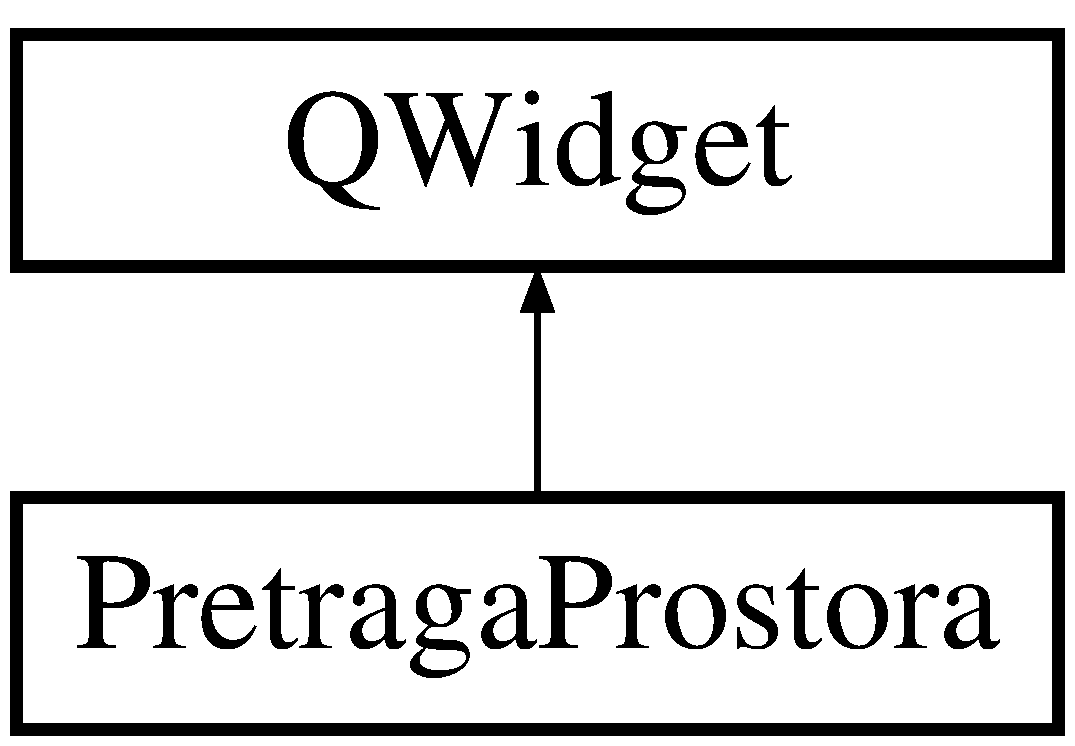
\includegraphics[height=2.000000cm]{class_pretraga_prostora}
\end{center}
\end{figure}
\subsection*{Signals}
\begin{DoxyCompactItemize}
\item 
void \hyperlink{class_pretraga_prostora_ab2120067abfe1b99db49c801859e2580}{jel\-Pretraga} (bool b)
\item 
void \hyperlink{class_pretraga_prostora_a2242f0fcbad64cd5a1d862eacc4b1075}{jel\-Crtanje} (bool b)
\end{DoxyCompactItemize}
\subsection*{Public Member Functions}
\begin{DoxyCompactItemize}
\item 
\hyperlink{class_pretraga_prostora_a9dcae5cdc25396e7c3d7d5800e40aa21}{Pretraga\-Prostora} (Q\-Widget $\ast$parent=0)
\begin{DoxyCompactList}\small\item\em Instanca klase stablo duzi. \end{DoxyCompactList}\item 
\hyperlink{class_pretraga_prostora_aec70c57efb108f48afd9b6a7bb1a51d5}{$\sim$\-Pretraga\-Prostora} ()
\item 
void \hyperlink{class_pretraga_prostora_a7d9629f10ac2734e46650cfe5d9e7678}{mouse\-Press\-Event} (Q\-Mouse\-Event $\ast$dogadjaj)
\item 
void \hyperlink{class_pretraga_prostora_aa829d10b5853ebec128e4ea5e8d9c50d}{mouse\-Move\-Event} (Q\-Mouse\-Event $\ast$dogadjaj)
\item 
void \hyperlink{class_pretraga_prostora_a824208ae98979eac421e98777269dd89}{mouse\-Release\-Event} (Q\-Mouse\-Event $\ast$dogadjaj)
\item 
void \hyperlink{class_pretraga_prostora_a1eae55313168c7878a04791904aca24d}{paint\-Event} (Q\-Paint\-Event $\ast$dogadjaj)
\item 
void \hyperlink{class_pretraga_prostora_a6d7560ae44bcc2346a73b84537d3e56e}{crtaj} (Q\-Painter $\ast$painter)
\item 
bool \hyperlink{class_pretraga_prostora_a77c67e48ced1ac4d64ba45fd091ed743}{kreiraj\-Iz\-Fajla} (Q\-String ime\-\_\-fajla)
\item 
bool \hyperlink{class_pretraga_prostora_a03158f7f63fe042715c1c87dd5030a9c}{spasi\-U\-Fajl} (Q\-String ime\-\_\-fajla)
\item 
void \hyperlink{class_pretraga_prostora_ad2c92c0d42c2a9c23788fcb352502e4c}{ponisti\-Odabir\-Duzi} ()
\end{DoxyCompactItemize}
\subsection*{Public Attributes}
\begin{DoxyCompactItemize}
\item 
\hyperlink{pretraga__raspona_8h_adc6e5733fc3c22f0a7b2914188c49c90}{state} \hyperlink{class_pretraga_prostora_ad93cf86ec7ba91d96f16c69ede98b180}{trenutno\-Stanje}
\item 
Q\-Point \hyperlink{class_pretraga_prostora_a1b67cf84d7be3e32d4d93bdd9ae14deb}{pocetak\-\_\-prozora}
\begin{DoxyCompactList}\small\item\em Trenutno stanje aplikacije. \end{DoxyCompactList}\item 
Q\-Point \hyperlink{class_pretraga_prostora_a5a852eb02e2b72c6a5d76c6014be973c}{start}
\begin{DoxyCompactList}\small\item\em Pocetna ta�ka prozora pretrage. \end{DoxyCompactList}\item 
Q\-Rubber\-Band $\ast$ \hyperlink{class_pretraga_prostora_a7ea1f4731d1530b881c09dc998c0b7eb}{izbor}
\begin{DoxyCompactList}\small\item\em Polazna ta�ka du�i u fazi kada ih kreiramo. \end{DoxyCompactList}\item 
Q\-Vector$<$ \hyperlink{struct_duz}{Duz} $>$ \hyperlink{class_pretraga_prostora_a71304ed78eb54bb4362e3f19b777b420}{vektor\-Duzi}
\begin{DoxyCompactList}\small\item\em Izabrani raspon. \end{DoxyCompactList}\item 
Q\-Vector$<$ \hyperlink{struct_krajnja_tacka_duzi}{Krajnja\-Tacka\-Duzi} $>$ \hyperlink{class_pretraga_prostora_a0757daf831ce7c8deae521e2bd56da3f}{vektor\-Krajnjih\-Tacaka}
\begin{DoxyCompactList}\small\item\em Vektor sa nacrtanim du�ima. \end{DoxyCompactList}\item 
Q\-Pen \hyperlink{class_pretraga_prostora_ae8c588bb3ba72d89da47ef6acb56d666}{crna}
\begin{DoxyCompactList}\small\item\em Vektor krajnjih ta�aka du�i \end{DoxyCompactList}\item 
Q\-Pen \hyperlink{class_pretraga_prostora_acc5253bae5ddafcd62073e8f88b21591}{crvena}
\begin{DoxyCompactList}\small\item\em Boja za oznacenu duzu. \end{DoxyCompactList}\item 
\hyperlink{class_stablo_raspona}{Stablo\-Raspona} \hyperlink{class_pretraga_prostora_a1aebe38ac90814aabf6de6eeae3930e4}{m\-\_\-rtree}
\begin{DoxyCompactList}\small\item\em Boja za neoznacenu duz. \end{DoxyCompactList}\item 
\hyperlink{class_stablo_duzi}{Stablo\-Duzi} \hyperlink{class_pretraga_prostora_a64f3f45de751ae06c41bb0f24d0d4850}{m\-\_\-stablo\-Duzi}
\begin{DoxyCompactList}\small\item\em Instanca klase stablo raspona. \end{DoxyCompactList}\end{DoxyCompactItemize}


\subsection{Detailed Description}


Definition at line 42 of file pretraga\-\_\-raspona.\-h.



\subsection{Constructor \& Destructor Documentation}
\hypertarget{class_pretraga_prostora_a9dcae5cdc25396e7c3d7d5800e40aa21}{\index{Pretraga\-Prostora@{Pretraga\-Prostora}!Pretraga\-Prostora@{Pretraga\-Prostora}}
\index{Pretraga\-Prostora@{Pretraga\-Prostora}!PretragaProstora@{Pretraga\-Prostora}}
\subsubsection[{Pretraga\-Prostora}]{\setlength{\rightskip}{0pt plus 5cm}Pretraga\-Prostora\-::\-Pretraga\-Prostora (
\begin{DoxyParamCaption}
\item[{Q\-Widget $\ast$}]{parent = {\ttfamily 0}}
\end{DoxyParamCaption}
)\hspace{0.3cm}{\ttfamily [explicit]}}}\label{class_pretraga_prostora_a9dcae5cdc25396e7c3d7d5800e40aa21}


Instanca klase stablo duzi. 



Definition at line 4 of file pretraga\-\_\-raspona.\-cpp.

\hypertarget{class_pretraga_prostora_aec70c57efb108f48afd9b6a7bb1a51d5}{\index{Pretraga\-Prostora@{Pretraga\-Prostora}!$\sim$\-Pretraga\-Prostora@{$\sim$\-Pretraga\-Prostora}}
\index{$\sim$\-Pretraga\-Prostora@{$\sim$\-Pretraga\-Prostora}!PretragaProstora@{Pretraga\-Prostora}}
\subsubsection[{$\sim$\-Pretraga\-Prostora}]{\setlength{\rightskip}{0pt plus 5cm}Pretraga\-Prostora\-::$\sim$\-Pretraga\-Prostora (
\begin{DoxyParamCaption}
{}
\end{DoxyParamCaption}
)}}\label{class_pretraga_prostora_aec70c57efb108f48afd9b6a7bb1a51d5}


Definition at line 14 of file pretraga\-\_\-raspona.\-cpp.



\subsection{Member Function Documentation}
\hypertarget{class_pretraga_prostora_a6d7560ae44bcc2346a73b84537d3e56e}{\index{Pretraga\-Prostora@{Pretraga\-Prostora}!crtaj@{crtaj}}
\index{crtaj@{crtaj}!PretragaProstora@{Pretraga\-Prostora}}
\subsubsection[{crtaj}]{\setlength{\rightskip}{0pt plus 5cm}void Pretraga\-Prostora\-::crtaj (
\begin{DoxyParamCaption}
\item[{Q\-Painter $\ast$}]{painter}
\end{DoxyParamCaption}
)}}\label{class_pretraga_prostora_a6d7560ae44bcc2346a73b84537d3e56e}


Definition at line 124 of file pretraga\-\_\-raspona.\-cpp.

\hypertarget{class_pretraga_prostora_a2242f0fcbad64cd5a1d862eacc4b1075}{\index{Pretraga\-Prostora@{Pretraga\-Prostora}!jel\-Crtanje@{jel\-Crtanje}}
\index{jel\-Crtanje@{jel\-Crtanje}!PretragaProstora@{Pretraga\-Prostora}}
\subsubsection[{jel\-Crtanje}]{\setlength{\rightskip}{0pt plus 5cm}void Pretraga\-Prostora\-::jel\-Crtanje (
\begin{DoxyParamCaption}
\item[{bool}]{b}
\end{DoxyParamCaption}
)\hspace{0.3cm}{\ttfamily [signal]}}}\label{class_pretraga_prostora_a2242f0fcbad64cd5a1d862eacc4b1075}


Definition at line 105 of file moc\-\_\-pretraga\-\_\-raspona.\-cpp.

\hypertarget{class_pretraga_prostora_ab2120067abfe1b99db49c801859e2580}{\index{Pretraga\-Prostora@{Pretraga\-Prostora}!jel\-Pretraga@{jel\-Pretraga}}
\index{jel\-Pretraga@{jel\-Pretraga}!PretragaProstora@{Pretraga\-Prostora}}
\subsubsection[{jel\-Pretraga}]{\setlength{\rightskip}{0pt plus 5cm}void Pretraga\-Prostora\-::jel\-Pretraga (
\begin{DoxyParamCaption}
\item[{bool}]{b}
\end{DoxyParamCaption}
)\hspace{0.3cm}{\ttfamily [signal]}}}\label{class_pretraga_prostora_ab2120067abfe1b99db49c801859e2580}


Definition at line 98 of file moc\-\_\-pretraga\-\_\-raspona.\-cpp.

\hypertarget{class_pretraga_prostora_a77c67e48ced1ac4d64ba45fd091ed743}{\index{Pretraga\-Prostora@{Pretraga\-Prostora}!kreiraj\-Iz\-Fajla@{kreiraj\-Iz\-Fajla}}
\index{kreiraj\-Iz\-Fajla@{kreiraj\-Iz\-Fajla}!PretragaProstora@{Pretraga\-Prostora}}
\subsubsection[{kreiraj\-Iz\-Fajla}]{\setlength{\rightskip}{0pt plus 5cm}bool Pretraga\-Prostora\-::kreiraj\-Iz\-Fajla (
\begin{DoxyParamCaption}
\item[{Q\-String}]{ime\-\_\-fajla}
\end{DoxyParamCaption}
)}}\label{class_pretraga_prostora_a77c67e48ced1ac4d64ba45fd091ed743}


Definition at line 143 of file pretraga\-\_\-raspona.\-cpp.

\hypertarget{class_pretraga_prostora_aa829d10b5853ebec128e4ea5e8d9c50d}{\index{Pretraga\-Prostora@{Pretraga\-Prostora}!mouse\-Move\-Event@{mouse\-Move\-Event}}
\index{mouse\-Move\-Event@{mouse\-Move\-Event}!PretragaProstora@{Pretraga\-Prostora}}
\subsubsection[{mouse\-Move\-Event}]{\setlength{\rightskip}{0pt plus 5cm}void Pretraga\-Prostora\-::mouse\-Move\-Event (
\begin{DoxyParamCaption}
\item[{Q\-Mouse\-Event $\ast$}]{dogadjaj}
\end{DoxyParamCaption}
)}}\label{class_pretraga_prostora_aa829d10b5853ebec128e4ea5e8d9c50d}


Definition at line 72 of file pretraga\-\_\-raspona.\-cpp.

\hypertarget{class_pretraga_prostora_a7d9629f10ac2734e46650cfe5d9e7678}{\index{Pretraga\-Prostora@{Pretraga\-Prostora}!mouse\-Press\-Event@{mouse\-Press\-Event}}
\index{mouse\-Press\-Event@{mouse\-Press\-Event}!PretragaProstora@{Pretraga\-Prostora}}
\subsubsection[{mouse\-Press\-Event}]{\setlength{\rightskip}{0pt plus 5cm}void Pretraga\-Prostora\-::mouse\-Press\-Event (
\begin{DoxyParamCaption}
\item[{Q\-Mouse\-Event $\ast$}]{dogadjaj}
\end{DoxyParamCaption}
)}}\label{class_pretraga_prostora_a7d9629f10ac2734e46650cfe5d9e7678}


Definition at line 26 of file pretraga\-\_\-raspona.\-cpp.

\hypertarget{class_pretraga_prostora_a824208ae98979eac421e98777269dd89}{\index{Pretraga\-Prostora@{Pretraga\-Prostora}!mouse\-Release\-Event@{mouse\-Release\-Event}}
\index{mouse\-Release\-Event@{mouse\-Release\-Event}!PretragaProstora@{Pretraga\-Prostora}}
\subsubsection[{mouse\-Release\-Event}]{\setlength{\rightskip}{0pt plus 5cm}void Pretraga\-Prostora\-::mouse\-Release\-Event (
\begin{DoxyParamCaption}
\item[{Q\-Mouse\-Event $\ast$}]{dogadjaj}
\end{DoxyParamCaption}
)}}\label{class_pretraga_prostora_a824208ae98979eac421e98777269dd89}


Definition at line 81 of file pretraga\-\_\-raspona.\-cpp.

\hypertarget{class_pretraga_prostora_a1eae55313168c7878a04791904aca24d}{\index{Pretraga\-Prostora@{Pretraga\-Prostora}!paint\-Event@{paint\-Event}}
\index{paint\-Event@{paint\-Event}!PretragaProstora@{Pretraga\-Prostora}}
\subsubsection[{paint\-Event}]{\setlength{\rightskip}{0pt plus 5cm}void Pretraga\-Prostora\-::paint\-Event (
\begin{DoxyParamCaption}
\item[{Q\-Paint\-Event $\ast$}]{dogadjaj}
\end{DoxyParamCaption}
)}}\label{class_pretraga_prostora_a1eae55313168c7878a04791904aca24d}


Definition at line 18 of file pretraga\-\_\-raspona.\-cpp.

\hypertarget{class_pretraga_prostora_ad2c92c0d42c2a9c23788fcb352502e4c}{\index{Pretraga\-Prostora@{Pretraga\-Prostora}!ponisti\-Odabir\-Duzi@{ponisti\-Odabir\-Duzi}}
\index{ponisti\-Odabir\-Duzi@{ponisti\-Odabir\-Duzi}!PretragaProstora@{Pretraga\-Prostora}}
\subsubsection[{ponisti\-Odabir\-Duzi}]{\setlength{\rightskip}{0pt plus 5cm}void Pretraga\-Prostora\-::ponisti\-Odabir\-Duzi (
\begin{DoxyParamCaption}
{}
\end{DoxyParamCaption}
)}}\label{class_pretraga_prostora_ad2c92c0d42c2a9c23788fcb352502e4c}


Definition at line 209 of file pretraga\-\_\-raspona.\-cpp.

\hypertarget{class_pretraga_prostora_a03158f7f63fe042715c1c87dd5030a9c}{\index{Pretraga\-Prostora@{Pretraga\-Prostora}!spasi\-U\-Fajl@{spasi\-U\-Fajl}}
\index{spasi\-U\-Fajl@{spasi\-U\-Fajl}!PretragaProstora@{Pretraga\-Prostora}}
\subsubsection[{spasi\-U\-Fajl}]{\setlength{\rightskip}{0pt plus 5cm}bool Pretraga\-Prostora\-::spasi\-U\-Fajl (
\begin{DoxyParamCaption}
\item[{Q\-String}]{ime\-\_\-fajla}
\end{DoxyParamCaption}
)}}\label{class_pretraga_prostora_a03158f7f63fe042715c1c87dd5030a9c}


Definition at line 181 of file pretraga\-\_\-raspona.\-cpp.



\subsection{Member Data Documentation}
\hypertarget{class_pretraga_prostora_ae8c588bb3ba72d89da47ef6acb56d666}{\index{Pretraga\-Prostora@{Pretraga\-Prostora}!crna@{crna}}
\index{crna@{crna}!PretragaProstora@{Pretraga\-Prostora}}
\subsubsection[{crna}]{\setlength{\rightskip}{0pt plus 5cm}Q\-Pen Pretraga\-Prostora\-::crna}}\label{class_pretraga_prostora_ae8c588bb3ba72d89da47ef6acb56d666}


Vektor krajnjih ta�aka du�i 



Definition at line 53 of file pretraga\-\_\-raspona.\-h.

\hypertarget{class_pretraga_prostora_acc5253bae5ddafcd62073e8f88b21591}{\index{Pretraga\-Prostora@{Pretraga\-Prostora}!crvena@{crvena}}
\index{crvena@{crvena}!PretragaProstora@{Pretraga\-Prostora}}
\subsubsection[{crvena}]{\setlength{\rightskip}{0pt plus 5cm}Q\-Pen Pretraga\-Prostora\-::crvena}}\label{class_pretraga_prostora_acc5253bae5ddafcd62073e8f88b21591}


Boja za oznacenu duzu. 



Definition at line 54 of file pretraga\-\_\-raspona.\-h.

\hypertarget{class_pretraga_prostora_a7ea1f4731d1530b881c09dc998c0b7eb}{\index{Pretraga\-Prostora@{Pretraga\-Prostora}!izbor@{izbor}}
\index{izbor@{izbor}!PretragaProstora@{Pretraga\-Prostora}}
\subsubsection[{izbor}]{\setlength{\rightskip}{0pt plus 5cm}Q\-Rubber\-Band$\ast$ Pretraga\-Prostora\-::izbor}}\label{class_pretraga_prostora_a7ea1f4731d1530b881c09dc998c0b7eb}


Polazna ta�ka du�i u fazi kada ih kreiramo. 



Definition at line 50 of file pretraga\-\_\-raspona.\-h.

\hypertarget{class_pretraga_prostora_a1aebe38ac90814aabf6de6eeae3930e4}{\index{Pretraga\-Prostora@{Pretraga\-Prostora}!m\-\_\-rtree@{m\-\_\-rtree}}
\index{m\-\_\-rtree@{m\-\_\-rtree}!PretragaProstora@{Pretraga\-Prostora}}
\subsubsection[{m\-\_\-rtree}]{\setlength{\rightskip}{0pt plus 5cm}{\bf Stablo\-Raspona} Pretraga\-Prostora\-::m\-\_\-rtree}}\label{class_pretraga_prostora_a1aebe38ac90814aabf6de6eeae3930e4}


Boja za neoznacenu duz. 



Definition at line 55 of file pretraga\-\_\-raspona.\-h.

\hypertarget{class_pretraga_prostora_a64f3f45de751ae06c41bb0f24d0d4850}{\index{Pretraga\-Prostora@{Pretraga\-Prostora}!m\-\_\-stablo\-Duzi@{m\-\_\-stablo\-Duzi}}
\index{m\-\_\-stablo\-Duzi@{m\-\_\-stablo\-Duzi}!PretragaProstora@{Pretraga\-Prostora}}
\subsubsection[{m\-\_\-stablo\-Duzi}]{\setlength{\rightskip}{0pt plus 5cm}{\bf Stablo\-Duzi} Pretraga\-Prostora\-::m\-\_\-stablo\-Duzi}}\label{class_pretraga_prostora_a64f3f45de751ae06c41bb0f24d0d4850}


Instanca klase stablo raspona. 



Definition at line 56 of file pretraga\-\_\-raspona.\-h.

\hypertarget{class_pretraga_prostora_a1b67cf84d7be3e32d4d93bdd9ae14deb}{\index{Pretraga\-Prostora@{Pretraga\-Prostora}!pocetak\-\_\-prozora@{pocetak\-\_\-prozora}}
\index{pocetak\-\_\-prozora@{pocetak\-\_\-prozora}!PretragaProstora@{Pretraga\-Prostora}}
\subsubsection[{pocetak\-\_\-prozora}]{\setlength{\rightskip}{0pt plus 5cm}Q\-Point Pretraga\-Prostora\-::pocetak\-\_\-prozora}}\label{class_pretraga_prostora_a1b67cf84d7be3e32d4d93bdd9ae14deb}


Trenutno stanje aplikacije. 



Definition at line 48 of file pretraga\-\_\-raspona.\-h.

\hypertarget{class_pretraga_prostora_a5a852eb02e2b72c6a5d76c6014be973c}{\index{Pretraga\-Prostora@{Pretraga\-Prostora}!start@{start}}
\index{start@{start}!PretragaProstora@{Pretraga\-Prostora}}
\subsubsection[{start}]{\setlength{\rightskip}{0pt plus 5cm}Q\-Point Pretraga\-Prostora\-::start}}\label{class_pretraga_prostora_a5a852eb02e2b72c6a5d76c6014be973c}


Pocetna ta�ka prozora pretrage. 



Definition at line 49 of file pretraga\-\_\-raspona.\-h.

\hypertarget{class_pretraga_prostora_ad93cf86ec7ba91d96f16c69ede98b180}{\index{Pretraga\-Prostora@{Pretraga\-Prostora}!trenutno\-Stanje@{trenutno\-Stanje}}
\index{trenutno\-Stanje@{trenutno\-Stanje}!PretragaProstora@{Pretraga\-Prostora}}
\subsubsection[{trenutno\-Stanje}]{\setlength{\rightskip}{0pt plus 5cm}{\bf state} Pretraga\-Prostora\-::trenutno\-Stanje}}\label{class_pretraga_prostora_ad93cf86ec7ba91d96f16c69ede98b180}


Definition at line 47 of file pretraga\-\_\-raspona.\-h.

\hypertarget{class_pretraga_prostora_a71304ed78eb54bb4362e3f19b777b420}{\index{Pretraga\-Prostora@{Pretraga\-Prostora}!vektor\-Duzi@{vektor\-Duzi}}
\index{vektor\-Duzi@{vektor\-Duzi}!PretragaProstora@{Pretraga\-Prostora}}
\subsubsection[{vektor\-Duzi}]{\setlength{\rightskip}{0pt plus 5cm}Q\-Vector$<${\bf Duz}$>$ Pretraga\-Prostora\-::vektor\-Duzi}}\label{class_pretraga_prostora_a71304ed78eb54bb4362e3f19b777b420}


Izabrani raspon. 



Definition at line 51 of file pretraga\-\_\-raspona.\-h.

\hypertarget{class_pretraga_prostora_a0757daf831ce7c8deae521e2bd56da3f}{\index{Pretraga\-Prostora@{Pretraga\-Prostora}!vektor\-Krajnjih\-Tacaka@{vektor\-Krajnjih\-Tacaka}}
\index{vektor\-Krajnjih\-Tacaka@{vektor\-Krajnjih\-Tacaka}!PretragaProstora@{Pretraga\-Prostora}}
\subsubsection[{vektor\-Krajnjih\-Tacaka}]{\setlength{\rightskip}{0pt plus 5cm}Q\-Vector$<${\bf Krajnja\-Tacka\-Duzi}$>$ Pretraga\-Prostora\-::vektor\-Krajnjih\-Tacaka}}\label{class_pretraga_prostora_a0757daf831ce7c8deae521e2bd56da3f}


Vektor sa nacrtanim du�ima. 



Definition at line 52 of file pretraga\-\_\-raspona.\-h.



The documentation for this class was generated from the following files\-:\begin{DoxyCompactItemize}
\item 
\hyperlink{pretraga__raspona_8h}{pretraga\-\_\-raspona.\-h}\item 
Generated\-Files/\-Debug/\hyperlink{_debug_2moc__pretraga__raspona_8cpp}{moc\-\_\-pretraga\-\_\-raspona.\-cpp}\item 
Generated\-Files/\-Release/\hyperlink{_release_2moc__pretraga__raspona_8cpp}{moc\-\_\-pretraga\-\_\-raspona.\-cpp}\item 
\hyperlink{pretraga__raspona_8cpp}{pretraga\-\_\-raspona.\-cpp}\end{DoxyCompactItemize}

\hypertarget{class_stablo_duzi}{\section{Stablo\-Duzi Class Reference}
\label{class_stablo_duzi}\index{Stablo\-Duzi@{Stablo\-Duzi}}
}


{\ttfamily \#include $<$stablo\-\_\-duzi.\-h$>$}

\subsection*{Public Member Functions}
\begin{DoxyCompactItemize}
\item 
\hyperlink{class_stablo_duzi_ae8ddb4ad40c367927b8956398e30bc5b}{Stablo\-Duzi} (Q\-Vector$<$ \hyperlink{struct_krajnja_tacka_duzi}{Krajnja\-Tacka\-Duzi} $>$ tacke, int dimenzija, Q\-Vector$<$ \hyperlink{struct_duz}{Duz} $>$ vek\-Duzi)
\item 
\hyperlink{class_stablo_duzi_aab221e06a3ce27fde8640ba1b5eec1f5}{Stablo\-Duzi} ()
\item 
void \hyperlink{class_stablo_duzi_a66092041df00427cc6c1318a9ce984b5}{pretrazi\-Stablo\-Duzi} (int ispitna\-\_\-vrijednost, int pocetak, int kraj, Q\-Vector$<$ \hyperlink{struct_duz}{Duz} $>$ \&vek\-Duzi, int dimenzija)
\end{DoxyCompactItemize}


\subsection{Detailed Description}


Definition at line 18 of file stablo\-\_\-duzi.\-h.



\subsection{Constructor \& Destructor Documentation}
\hypertarget{class_stablo_duzi_ae8ddb4ad40c367927b8956398e30bc5b}{\index{Stablo\-Duzi@{Stablo\-Duzi}!Stablo\-Duzi@{Stablo\-Duzi}}
\index{Stablo\-Duzi@{Stablo\-Duzi}!StabloDuzi@{Stablo\-Duzi}}
\subsubsection[{Stablo\-Duzi}]{\setlength{\rightskip}{0pt plus 5cm}Stablo\-Duzi\-::\-Stablo\-Duzi (
\begin{DoxyParamCaption}
\item[{Q\-Vector$<$ {\bf Krajnja\-Tacka\-Duzi} $>$}]{tacke, }
\item[{int}]{dimenzija, }
\item[{Q\-Vector$<$ {\bf Duz} $>$}]{vek\-Duzi}
\end{DoxyParamCaption}
)}}\label{class_stablo_duzi_ae8ddb4ad40c367927b8956398e30bc5b}


Definition at line 3 of file stablo\-\_\-duzi.\-cpp.

\hypertarget{class_stablo_duzi_aab221e06a3ce27fde8640ba1b5eec1f5}{\index{Stablo\-Duzi@{Stablo\-Duzi}!Stablo\-Duzi@{Stablo\-Duzi}}
\index{Stablo\-Duzi@{Stablo\-Duzi}!StabloDuzi@{Stablo\-Duzi}}
\subsubsection[{Stablo\-Duzi}]{\setlength{\rightskip}{0pt plus 5cm}Stablo\-Duzi\-::\-Stablo\-Duzi (
\begin{DoxyParamCaption}
{}
\end{DoxyParamCaption}
)\hspace{0.3cm}{\ttfamily [inline]}}}\label{class_stablo_duzi_aab221e06a3ce27fde8640ba1b5eec1f5}


Definition at line 226 of file stablo\-\_\-duzi.\-h.



\subsection{Member Function Documentation}
\hypertarget{class_stablo_duzi_a66092041df00427cc6c1318a9ce984b5}{\index{Stablo\-Duzi@{Stablo\-Duzi}!pretrazi\-Stablo\-Duzi@{pretrazi\-Stablo\-Duzi}}
\index{pretrazi\-Stablo\-Duzi@{pretrazi\-Stablo\-Duzi}!StabloDuzi@{Stablo\-Duzi}}
\subsubsection[{pretrazi\-Stablo\-Duzi}]{\setlength{\rightskip}{0pt plus 5cm}void Stablo\-Duzi\-::pretrazi\-Stablo\-Duzi (
\begin{DoxyParamCaption}
\item[{int}]{ispitna\-\_\-vrijednost, }
\item[{int}]{pocetak, }
\item[{int}]{kraj, }
\item[{Q\-Vector$<$ {\bf Duz} $>$ \&}]{vek\-Duzi, }
\item[{int}]{dimenzija}
\end{DoxyParamCaption}
)}}\label{class_stablo_duzi_a66092041df00427cc6c1318a9ce984b5}


Definition at line 429 of file stablo\-\_\-duzi.\-cpp.



The documentation for this class was generated from the following files\-:\begin{DoxyCompactItemize}
\item 
\hyperlink{stablo__duzi_8h}{stablo\-\_\-duzi.\-h}\item 
\hyperlink{stablo__duzi_8cpp}{stablo\-\_\-duzi.\-cpp}\end{DoxyCompactItemize}

\hypertarget{class_stablo_raspona}{\section{Stablo\-Raspona Class Reference}
\label{class_stablo_raspona}\index{Stablo\-Raspona@{Stablo\-Raspona}}
}


{\ttfamily \#include $<$stablo\-\_\-raspona.\-h$>$}

\subsection*{Public Types}
\begin{DoxyCompactItemize}
\item 
typedef boost\-::shared\-\_\-ptr$<$ Cvor $>$ \hyperlink{class_stablo_raspona_ab8a758e341c6a09c482bd3802c3eb6e8}{p\-Cvor}
\end{DoxyCompactItemize}
\subsection*{Public Member Functions}
\begin{DoxyCompactItemize}
\item 
\hyperlink{class_stablo_raspona_ad4ed5d791e2b8adb6563cff8b55544c5}{Stablo\-Raspona} ()
\item 
\hyperlink{class_stablo_raspona_abbdeacd2b1807bb4cdc524e651d2c80a}{Stablo\-Raspona} (Q\-Vector$<$ \hyperlink{struct_krajnja_tacka_duzi}{Krajnja\-Tacka\-Duzi} $>$ tacke, int dimenzija)
\item 
void \hyperlink{class_stablo_raspona_aba64a9f4197752410506cd514bb80f53}{pretraga\-Raspona} (int x1, int x2, int y1, int y2)
\item 
Q\-Vector$<$ \hyperlink{struct_krajnja_tacka_duzi}{Krajnja\-Tacka\-Duzi} $>$ \hyperlink{class_stablo_raspona_aa4426f8f780183052feedc79721648c3}{daj\-Rezultat} ()
\item 
\hyperlink{class_stablo_raspona_ad4ed5d791e2b8adb6563cff8b55544c5}{Stablo\-Raspona} ()
\item 
\hyperlink{class_stablo_raspona_abbdeacd2b1807bb4cdc524e651d2c80a}{Stablo\-Raspona} (Q\-Vector$<$ \hyperlink{struct_krajnja_tacka_duzi}{Krajnja\-Tacka\-Duzi} $>$ tacke, int dimenzija)
\item 
void \hyperlink{class_stablo_raspona_ab15582f7f4c015c21295b4957cfd49a7}{pretraga\-Raspona} (\hyperlink{struct_krajnja_tacka_duzi}{Krajnja\-Tacka\-Duzi} pocetak, \hyperlink{struct_krajnja_tacka_duzi}{Krajnja\-Tacka\-Duzi} kraj, int dim)
\item 
Q\-Vector$<$ \hyperlink{struct_krajnja_tacka_duzi}{Krajnja\-Tacka\-Duzi} $>$ \hyperlink{class_stablo_raspona_af93cb0b9ee1ca56fe1682281df955f03}{vrati\-Rezultat} ()
\end{DoxyCompactItemize}


\subsection{Detailed Description}


Definition at line 16 of file stablo\-\_\-raspona.\-h.



\subsection{Member Typedef Documentation}
\hypertarget{class_stablo_raspona_ab8a758e341c6a09c482bd3802c3eb6e8}{\index{Stablo\-Raspona@{Stablo\-Raspona}!p\-Cvor@{p\-Cvor}}
\index{p\-Cvor@{p\-Cvor}!StabloRaspona@{Stablo\-Raspona}}
\subsubsection[{p\-Cvor}]{\setlength{\rightskip}{0pt plus 5cm}typedef boost\-::shared\-\_\-ptr$<$Cvor$>$ {\bf Stablo\-Raspona\-::p\-Cvor}}}\label{class_stablo_raspona_ab8a758e341c6a09c482bd3802c3eb6e8}


Definition at line 32 of file stablo\-\_\-raspona.\-h.



\subsection{Constructor \& Destructor Documentation}
\hypertarget{class_stablo_raspona_ad4ed5d791e2b8adb6563cff8b55544c5}{\index{Stablo\-Raspona@{Stablo\-Raspona}!Stablo\-Raspona@{Stablo\-Raspona}}
\index{Stablo\-Raspona@{Stablo\-Raspona}!StabloRaspona@{Stablo\-Raspona}}
\subsubsection[{Stablo\-Raspona}]{\setlength{\rightskip}{0pt plus 5cm}Stablo\-Raspona\-::\-Stablo\-Raspona (
\begin{DoxyParamCaption}
{}
\end{DoxyParamCaption}
)}}\label{class_stablo_raspona_ad4ed5d791e2b8adb6563cff8b55544c5}


Definition at line 16 of file stablo\-\_\-raspona.\-cpp.

\hypertarget{class_stablo_raspona_abbdeacd2b1807bb4cdc524e651d2c80a}{\index{Stablo\-Raspona@{Stablo\-Raspona}!Stablo\-Raspona@{Stablo\-Raspona}}
\index{Stablo\-Raspona@{Stablo\-Raspona}!StabloRaspona@{Stablo\-Raspona}}
\subsubsection[{Stablo\-Raspona}]{\setlength{\rightskip}{0pt plus 5cm}Stablo\-Raspona\-::\-Stablo\-Raspona (
\begin{DoxyParamCaption}
\item[{Q\-Vector$<$ {\bf Krajnja\-Tacka\-Duzi} $>$}]{tacke, }
\item[{int}]{dimenzija}
\end{DoxyParamCaption}
)}}\label{class_stablo_raspona_abbdeacd2b1807bb4cdc524e651d2c80a}
@ brief Konstruktor Stabla Raspona


\begin{DoxyParams}[1]{Parameters}
\mbox{\tt in}  & {\em tacke} & vektor kranjih ta�aka du�i koje �emo pretraziti \\
\hline
\mbox{\tt in}  & {\em dimenzija} & u kojoj �emo stablo raspona napraviti \\
\hline
\end{DoxyParams}


Definition at line 10 of file stablo\-\_\-raspona.\-cpp.

\hypertarget{class_stablo_raspona_ad4ed5d791e2b8adb6563cff8b55544c5}{\index{Stablo\-Raspona@{Stablo\-Raspona}!Stablo\-Raspona@{Stablo\-Raspona}}
\index{Stablo\-Raspona@{Stablo\-Raspona}!StabloRaspona@{Stablo\-Raspona}}
\subsubsection[{Stablo\-Raspona}]{\setlength{\rightskip}{0pt plus 5cm}Stablo\-Raspona\-::\-Stablo\-Raspona (
\begin{DoxyParamCaption}
{}
\end{DoxyParamCaption}
)}}\label{class_stablo_raspona_ad4ed5d791e2b8adb6563cff8b55544c5}
\hypertarget{class_stablo_raspona_abbdeacd2b1807bb4cdc524e651d2c80a}{\index{Stablo\-Raspona@{Stablo\-Raspona}!Stablo\-Raspona@{Stablo\-Raspona}}
\index{Stablo\-Raspona@{Stablo\-Raspona}!StabloRaspona@{Stablo\-Raspona}}
\subsubsection[{Stablo\-Raspona}]{\setlength{\rightskip}{0pt plus 5cm}Stablo\-Raspona\-::\-Stablo\-Raspona (
\begin{DoxyParamCaption}
\item[{Q\-Vector$<$ {\bf Krajnja\-Tacka\-Duzi} $>$}]{tacke, }
\item[{int}]{dimenzija}
\end{DoxyParamCaption}
)}}\label{class_stablo_raspona_abbdeacd2b1807bb4cdc524e651d2c80a}


\subsection{Member Function Documentation}
\hypertarget{class_stablo_raspona_aa4426f8f780183052feedc79721648c3}{\index{Stablo\-Raspona@{Stablo\-Raspona}!daj\-Rezultat@{daj\-Rezultat}}
\index{daj\-Rezultat@{daj\-Rezultat}!StabloRaspona@{Stablo\-Raspona}}
\subsubsection[{daj\-Rezultat}]{\setlength{\rightskip}{0pt plus 5cm}Q\-Vector$<${\bf Krajnja\-Tacka\-Duzi}$>$ Stablo\-Raspona\-::daj\-Rezultat (
\begin{DoxyParamCaption}
{}
\end{DoxyParamCaption}
)\hspace{0.3cm}{\ttfamily [inline]}}}\label{class_stablo_raspona_aa4426f8f780183052feedc79721648c3}


Definition at line 51 of file stablo\-\_\-raspona.\-h.

\hypertarget{class_stablo_raspona_aba64a9f4197752410506cd514bb80f53}{\index{Stablo\-Raspona@{Stablo\-Raspona}!pretraga\-Raspona@{pretraga\-Raspona}}
\index{pretraga\-Raspona@{pretraga\-Raspona}!StabloRaspona@{Stablo\-Raspona}}
\subsubsection[{pretraga\-Raspona}]{\setlength{\rightskip}{0pt plus 5cm}void Stablo\-Raspona\-::pretraga\-Raspona (
\begin{DoxyParamCaption}
\item[{int}]{x1, }
\item[{int}]{x2, }
\item[{int}]{y1, }
\item[{int}]{y2}
\end{DoxyParamCaption}
)}}\label{class_stablo_raspona_aba64a9f4197752410506cd514bb80f53}


Definition at line 131 of file stablo\-\_\-raspona.\-cpp.

\hypertarget{class_stablo_raspona_ab15582f7f4c015c21295b4957cfd49a7}{\index{Stablo\-Raspona@{Stablo\-Raspona}!pretraga\-Raspona@{pretraga\-Raspona}}
\index{pretraga\-Raspona@{pretraga\-Raspona}!StabloRaspona@{Stablo\-Raspona}}
\subsubsection[{pretraga\-Raspona}]{\setlength{\rightskip}{0pt plus 5cm}void Stablo\-Raspona\-::pretraga\-Raspona (
\begin{DoxyParamCaption}
\item[{{\bf Krajnja\-Tacka\-Duzi}}]{pocetak, }
\item[{{\bf Krajnja\-Tacka\-Duzi}}]{kraj, }
\item[{int}]{dim}
\end{DoxyParamCaption}
)}}\label{class_stablo_raspona_ab15582f7f4c015c21295b4957cfd49a7}


Definition at line 95 of file stablo\-\_\-raspona.\-cpp.

\hypertarget{class_stablo_raspona_af93cb0b9ee1ca56fe1682281df955f03}{\index{Stablo\-Raspona@{Stablo\-Raspona}!vrati\-Rezultat@{vrati\-Rezultat}}
\index{vrati\-Rezultat@{vrati\-Rezultat}!StabloRaspona@{Stablo\-Raspona}}
\subsubsection[{vrati\-Rezultat}]{\setlength{\rightskip}{0pt plus 5cm}Q\-Vector$<${\bf Krajnja\-Tacka\-Duzi}$>$ Stablo\-Raspona\-::vrati\-Rezultat (
\begin{DoxyParamCaption}
{}
\end{DoxyParamCaption}
)\hspace{0.3cm}{\ttfamily [inline]}}}\label{class_stablo_raspona_af93cb0b9ee1ca56fe1682281df955f03}


Definition at line 138 of file stablo\-\_\-raspona.\-h.



The documentation for this class was generated from the following files\-:\begin{DoxyCompactItemize}
\item 
backup/\hyperlink{backup_2stablo__raspona_8h}{stablo\-\_\-raspona.\-h}\item 
\hyperlink{stablo__raspona_8h}{stablo\-\_\-raspona.\-h}\item 
backup/\hyperlink{backup_2stablo__raspona_8cpp}{stablo\-\_\-raspona.\-cpp}\item 
\hyperlink{stablo__raspona_8cpp}{stablo\-\_\-raspona.\-cpp}\end{DoxyCompactItemize}

\chapter{File Documentation}
\hypertarget{backup_2stablo__raspona_8cpp}{\section{backup/stablo\-\_\-raspona.cpp File Reference}
\label{backup_2stablo__raspona_8cpp}\index{backup/stablo\-\_\-raspona.\-cpp@{backup/stablo\-\_\-raspona.\-cpp}}
}
{\ttfamily \#include \char`\"{}stablo\-\_\-raspona.\-h\char`\"{}}\\*

\hypertarget{stablo__raspona_8cpp}{\section{stablo\-\_\-raspona.\-cpp File Reference}
\label{stablo__raspona_8cpp}\index{stablo\-\_\-raspona.\-cpp@{stablo\-\_\-raspona.\-cpp}}
}
{\ttfamily \#include \char`\"{}stablo\-\_\-raspona.\-h\char`\"{}}\\*

\hypertarget{backup_2stablo__raspona_8h}{\section{backup/stablo\-\_\-raspona.h File Reference}
\label{backup_2stablo__raspona_8h}\index{backup/stablo\-\_\-raspona.\-h@{backup/stablo\-\_\-raspona.\-h}}
}
{\ttfamily \#include $<$vector$>$}\\*
{\ttfamily \#include $<$algorithm$>$}\\*
{\ttfamily \#include $<$boost/foreach.\-hpp$>$}\\*
{\ttfamily \#include $<$boost/shared\-\_\-ptr.\-hpp$>$}\\*
{\ttfamily \#include \char`\"{}strukture.\-h\char`\"{}}\\*
\subsection*{Classes}
\begin{DoxyCompactItemize}
\item 
class \hyperlink{class_stablo_raspona}{Stablo\-Raspona}
\end{DoxyCompactItemize}

\hypertarget{stablo__raspona_8h}{\section{stablo\-\_\-raspona.\-h File Reference}
\label{stablo__raspona_8h}\index{stablo\-\_\-raspona.\-h@{stablo\-\_\-raspona.\-h}}
}
{\ttfamily \#include $<$Q\-Vector$>$}\\*
{\ttfamily \#include $<$algorithm$>$}\\*
{\ttfamily \#include $<$boost/foreach.\-hpp$>$}\\*
{\ttfamily \#include $<$boost/shared\-\_\-ptr.\-hpp$>$}\\*
{\ttfamily \#include \char`\"{}strukture.\-h\char`\"{}}\\*
\subsection*{Classes}
\begin{DoxyCompactItemize}
\item 
class \hyperlink{class_stablo_raspona}{Stablo\-Raspona}
\end{DoxyCompactItemize}

\hypertarget{backup_2strukture_8h}{\section{backup/strukture.h File Reference}
\label{backup_2strukture_8h}\index{backup/strukture.\-h@{backup/strukture.\-h}}
}
{\ttfamily \#include $<$Q\-Point$>$}\\*
{\ttfamily \#include $<$Q\-Vector$>$}\\*
\subsection*{Classes}
\begin{DoxyCompactItemize}
\item 
struct \hyperlink{struct_duz}{Duz}
\item 
struct \hyperlink{struct_krajnja_tacka_duzi}{Krajnja\-Tacka\-Duzi}
\item 
struct \hyperlink{struct_elementarni_interval}{Elementarni\-Interval}
\item 
struct \hyperlink{struct_poredjenje_po_x}{Poredjenje\-Po\-X}
\item 
struct \hyperlink{struct_poredjenje_po_y}{Poredjenje\-Po\-Y}
\end{DoxyCompactItemize}

\hypertarget{strukture_8h}{\section{strukture.\-h File Reference}
\label{strukture_8h}\index{strukture.\-h@{strukture.\-h}}
}
{\ttfamily \#include $<$Q\-Point$>$}\\*
{\ttfamily \#include $<$Q\-Vector$>$}\\*
\subsection*{Classes}
\begin{DoxyCompactItemize}
\item 
struct \hyperlink{struct_duz}{Duz}
\item 
struct \hyperlink{struct_krajnja_tacka_duzi}{Krajnja\-Tacka\-Duzi}
\item 
struct \hyperlink{struct_elementarni_interval}{Elementarni\-Interval}
\item 
struct \hyperlink{struct_poredjenje_po_x}{Poredjenje\-Po\-X}
\item 
struct \hyperlink{struct_poredjenje_po_y}{Poredjenje\-Po\-Y}
\end{DoxyCompactItemize}

\hypertarget{_debug_2moc__pretraga__raspona_8cpp}{\section{Generated\-Files/\-Debug/moc\-\_\-pretraga\-\_\-raspona.cpp File Reference}
\label{_debug_2moc__pretraga__raspona_8cpp}\index{Generated\-Files/\-Debug/moc\-\_\-pretraga\-\_\-raspona.\-cpp@{Generated\-Files/\-Debug/moc\-\_\-pretraga\-\_\-raspona.\-cpp}}
}
{\ttfamily \#include \char`\"{}../../pretraga\-\_\-raspona.\-h\char`\"{}}\\*

\hypertarget{_release_2moc__pretraga__raspona_8cpp}{\section{Generated\-Files/\-Release/moc\-\_\-pretraga\-\_\-raspona.cpp File Reference}
\label{_release_2moc__pretraga__raspona_8cpp}\index{Generated\-Files/\-Release/moc\-\_\-pretraga\-\_\-raspona.\-cpp@{Generated\-Files/\-Release/moc\-\_\-pretraga\-\_\-raspona.\-cpp}}
}
{\ttfamily \#include \char`\"{}../../pretraga\-\_\-raspona.\-h\char`\"{}}\\*

\hypertarget{qrc__resursi_8cpp}{\section{Generated\-Files/qrc\-\_\-resursi.cpp File Reference}
\label{qrc__resursi_8cpp}\index{Generated\-Files/qrc\-\_\-resursi.\-cpp@{Generated\-Files/qrc\-\_\-resursi.\-cpp}}
}
{\ttfamily \#include $<$Qt\-Core/qglobal.\-h$>$}\\*
\subsection*{Functions}
\begin{DoxyCompactItemize}
\item 
Q\-T\-\_\-\-B\-E\-G\-I\-N\-\_\-\-N\-A\-M\-E\-S\-P\-A\-C\-E \\*
Q\-\_\-\-C\-O\-R\-E\-\_\-\-E\-X\-P\-O\-R\-T bool \hyperlink{qrc__resursi_8cpp_ab3bec3d1e679084be46edc41e4c91bc1}{q\-Register\-Resource\-Data} (int, const unsigned char $\ast$, const unsigned char $\ast$, const unsigned char $\ast$)
\item 
Q\-\_\-\-C\-O\-R\-E\-\_\-\-E\-X\-P\-O\-R\-T bool \hyperlink{qrc__resursi_8cpp_ad65f8bca8010dd1fd135a28a085c6d03}{q\-Unregister\-Resource\-Data} (int, const unsigned char $\ast$, const unsigned char $\ast$, const unsigned char $\ast$)
\item 
Q\-T\-\_\-\-E\-N\-D\-\_\-\-N\-A\-M\-E\-S\-P\-A\-C\-E int \\*
Q\-T\-\_\-\-M\-A\-N\-G\-L\-E\-\_\-\-N\-A\-M\-E\-S\-P\-A\-C\-E() \hyperlink{qrc__resursi_8cpp_a7b35bc57a944d036535e69a0058ba0d0}{q\-Init\-Resources\-\_\-resursi} ()
\item 
int Q\-T\-\_\-\-M\-A\-N\-G\-L\-E\-\_\-\-N\-A\-M\-E\-S\-P\-A\-C\-E() \hyperlink{qrc__resursi_8cpp_a77772f4e0b801c259a205e9b0f0d70dc}{q\-Cleanup\-Resources\-\_\-resursi} ()
\end{DoxyCompactItemize}


\subsection{Function Documentation}
\hypertarget{qrc__resursi_8cpp_a77772f4e0b801c259a205e9b0f0d70dc}{\index{qrc\-\_\-resursi.\-cpp@{qrc\-\_\-resursi.\-cpp}!q\-Cleanup\-Resources\-\_\-resursi@{q\-Cleanup\-Resources\-\_\-resursi}}
\index{q\-Cleanup\-Resources\-\_\-resursi@{q\-Cleanup\-Resources\-\_\-resursi}!qrc_resursi.cpp@{qrc\-\_\-resursi.\-cpp}}
\subsubsection[{q\-Cleanup\-Resources\-\_\-resursi}]{\setlength{\rightskip}{0pt plus 5cm}int Q\-T\-\_\-\-M\-A\-N\-G\-L\-E\-\_\-\-N\-A\-M\-E\-S\-P\-A\-C\-E() q\-Cleanup\-Resources\-\_\-resursi (
\begin{DoxyParamCaption}
{}
\end{DoxyParamCaption}
)}}\label{qrc__resursi_8cpp_a77772f4e0b801c259a205e9b0f0d70dc}


Definition at line 1058 of file qrc\-\_\-resursi.\-cpp.

\hypertarget{qrc__resursi_8cpp_a7b35bc57a944d036535e69a0058ba0d0}{\index{qrc\-\_\-resursi.\-cpp@{qrc\-\_\-resursi.\-cpp}!q\-Init\-Resources\-\_\-resursi@{q\-Init\-Resources\-\_\-resursi}}
\index{q\-Init\-Resources\-\_\-resursi@{q\-Init\-Resources\-\_\-resursi}!qrc_resursi.cpp@{qrc\-\_\-resursi.\-cpp}}
\subsubsection[{q\-Init\-Resources\-\_\-resursi}]{\setlength{\rightskip}{0pt plus 5cm}Q\-T\-\_\-\-E\-N\-D\-\_\-\-N\-A\-M\-E\-S\-P\-A\-C\-E int Q\-T\-\_\-\-M\-A\-N\-G\-L\-E\-\_\-\-N\-A\-M\-E\-S\-P\-A\-C\-E() q\-Init\-Resources\-\_\-resursi (
\begin{DoxyParamCaption}
{}
\end{DoxyParamCaption}
)}}\label{qrc__resursi_8cpp_a7b35bc57a944d036535e69a0058ba0d0}


Definition at line 1049 of file qrc\-\_\-resursi.\-cpp.

\hypertarget{qrc__resursi_8cpp_ab3bec3d1e679084be46edc41e4c91bc1}{\index{qrc\-\_\-resursi.\-cpp@{qrc\-\_\-resursi.\-cpp}!q\-Register\-Resource\-Data@{q\-Register\-Resource\-Data}}
\index{q\-Register\-Resource\-Data@{q\-Register\-Resource\-Data}!qrc_resursi.cpp@{qrc\-\_\-resursi.\-cpp}}
\subsubsection[{q\-Register\-Resource\-Data}]{\setlength{\rightskip}{0pt plus 5cm}Q\-T\-\_\-\-B\-E\-G\-I\-N\-\_\-\-N\-A\-M\-E\-S\-P\-A\-C\-E Q\-\_\-\-C\-O\-R\-E\-\_\-\-E\-X\-P\-O\-R\-T bool q\-Register\-Resource\-Data (
\begin{DoxyParamCaption}
\item[{int}]{, }
\item[{const unsigned char $\ast$}]{, }
\item[{const unsigned char $\ast$}]{, }
\item[{const unsigned char $\ast$}]{}
\end{DoxyParamCaption}
)}}\label{qrc__resursi_8cpp_ab3bec3d1e679084be46edc41e4c91bc1}
\hypertarget{qrc__resursi_8cpp_ad65f8bca8010dd1fd135a28a085c6d03}{\index{qrc\-\_\-resursi.\-cpp@{qrc\-\_\-resursi.\-cpp}!q\-Unregister\-Resource\-Data@{q\-Unregister\-Resource\-Data}}
\index{q\-Unregister\-Resource\-Data@{q\-Unregister\-Resource\-Data}!qrc_resursi.cpp@{qrc\-\_\-resursi.\-cpp}}
\subsubsection[{q\-Unregister\-Resource\-Data}]{\setlength{\rightskip}{0pt plus 5cm}Q\-\_\-\-C\-O\-R\-E\-\_\-\-E\-X\-P\-O\-R\-T bool q\-Unregister\-Resource\-Data (
\begin{DoxyParamCaption}
\item[{int}]{, }
\item[{const unsigned char $\ast$}]{, }
\item[{const unsigned char $\ast$}]{, }
\item[{const unsigned char $\ast$}]{}
\end{DoxyParamCaption}
)}}\label{qrc__resursi_8cpp_ad65f8bca8010dd1fd135a28a085c6d03}

\hypertarget{main_8cpp}{\section{main.\-cpp File Reference}
\label{main_8cpp}\index{main.\-cpp@{main.\-cpp}}
}
{\ttfamily \#include $<$Qt\-Gui/\-Q\-Application$>$}\\*
{\ttfamily \#include \char`\"{}pretraga\-\_\-raspona.\-h\char`\"{}}\\*
\subsection*{Functions}
\begin{DoxyCompactItemize}
\item 
int \hyperlink{main_8cpp_a0ddf1224851353fc92bfbff6f499fa97}{main} (int argc, char $\ast$argv\mbox{[}$\,$\mbox{]})
\end{DoxyCompactItemize}


\subsection{Function Documentation}
\hypertarget{main_8cpp_a0ddf1224851353fc92bfbff6f499fa97}{\index{main.\-cpp@{main.\-cpp}!main@{main}}
\index{main@{main}!main.cpp@{main.\-cpp}}
\subsubsection[{main}]{\setlength{\rightskip}{0pt plus 5cm}int main (
\begin{DoxyParamCaption}
\item[{int}]{argc, }
\item[{char $\ast$}]{argv\mbox{[}$\,$\mbox{]}}
\end{DoxyParamCaption}
)}}\label{main_8cpp_a0ddf1224851353fc92bfbff6f499fa97}


Definition at line 4 of file main.\-cpp.


\hypertarget{pretraga__raspona_8cpp}{\section{pretraga\-\_\-raspona.\-cpp File Reference}
\label{pretraga__raspona_8cpp}\index{pretraga\-\_\-raspona.\-cpp@{pretraga\-\_\-raspona.\-cpp}}
}
{\ttfamily \#include \char`\"{}pretraga\-\_\-raspona.\-h\char`\"{}}\\*

\hypertarget{pretraga__raspona_8h}{\section{pretraga\-\_\-raspona.\-h File Reference}
\label{pretraga__raspona_8h}\index{pretraga\-\_\-raspona.\-h@{pretraga\-\_\-raspona.\-h}}
}
{\ttfamily \#include $<$iostream$>$}\\*
{\ttfamily \#include $<$Q\-Text\-Stream$>$}\\*
{\ttfamily \#include $<$Q\-Vector$>$}\\*
{\ttfamily \#include $<$Q\-Vector\-Iterator$>$}\\*
{\ttfamily \#include \char`\"{}strukture.\-h\char`\"{}}\\*
{\ttfamily \#include $<$Q\-File\-Dialog$>$}\\*
{\ttfamily \#include $<$Q\-Painter$>$}\\*
{\ttfamily \#include $<$Q\-Point$>$}\\*
{\ttfamily \#include $<$Q\-Rubber\-Band$>$}\\*
{\ttfamily \#include $<$Q\-Mouse\-Event$>$}\\*
{\ttfamily \#include $<$Q\-Message\-Box$>$}\\*
{\ttfamily \#include $<$Qt\-Core/\-Q\-Variant$>$}\\*
{\ttfamily \#include $<$Qt\-Gui/\-Q\-Action$>$}\\*
{\ttfamily \#include $<$Qt\-Gui/\-Q\-Application$>$}\\*
{\ttfamily \#include $<$Qt\-Gui/\-Q\-Button\-Group$>$}\\*
{\ttfamily \#include $<$Qt\-Gui/\-Q\-Header\-View$>$}\\*
{\ttfamily \#include $<$Qt\-Gui/\-Q\-Main\-Window$>$}\\*
{\ttfamily \#include $<$Qt\-Gui/\-Q\-Menu$>$}\\*
{\ttfamily \#include $<$Qt\-Gui/\-Q\-Menu\-Bar$>$}\\*
{\ttfamily \#include $<$Qt\-Gui/\-Q\-Status\-Bar$>$}\\*
{\ttfamily \#include $<$Qt\-Gui/\-Q\-Tool\-Bar$>$}\\*
{\ttfamily \#include $<$Qt\-Gui/\-Q\-Widget$>$}\\*
{\ttfamily \#include $<$Qt\-Algorithms$>$}\\*
{\ttfamily \#include $<$math.\-h$>$}\\*
{\ttfamily \#include \char`\"{}stablo\-\_\-raspona.\-h\char`\"{}}\\*
{\ttfamily \#include \char`\"{}stablo\-\_\-duzi.\-h\char`\"{}}\\*
\subsection*{Classes}
\begin{DoxyCompactItemize}
\item 
class \hyperlink{class_pretraga_prostora}{Pretraga\-Prostora}
\end{DoxyCompactItemize}
\subsection*{Macros}
\begin{DoxyCompactItemize}
\item 
\#define \hyperlink{pretraga__raspona_8h_a2cc1a627c7d1839b4492a459c6ea6a73}{N\-E\-G\-B\-E\-S\-K\-O\-N\-A\-C\-N\-O}~-\/5000
\item 
\#define \hyperlink{pretraga__raspona_8h_a8474b48b668a74c16680425865ee9658}{P\-O\-Z\-B\-E\-S\-K\-O\-N\-A\-C\-N\-O}~+5000
\end{DoxyCompactItemize}
\subsection*{Enumerations}
\begin{DoxyCompactItemize}
\item 
enum \hyperlink{pretraga__raspona_8h_adc6e5733fc3c22f0a7b2914188c49c90}{state} \{ \hyperlink{pretraga__raspona_8h_adc6e5733fc3c22f0a7b2914188c49c90a80ccf7e839fca4f0c3e059f2937d5d79}{C\-E\-K\-A\-N\-J\-A}, 
\hyperlink{pretraga__raspona_8h_adc6e5733fc3c22f0a7b2914188c49c90af189cfaa8f64bfe3679bc5ab3338d537}{P\-R\-E\-T\-R\-A\-G\-A}, 
\hyperlink{pretraga__raspona_8h_adc6e5733fc3c22f0a7b2914188c49c90af04dc3fd7d286e3b2f0d47d9af522b7d}{C\-R\-T\-A\-N\-J\-A1}, 
\hyperlink{pretraga__raspona_8h_adc6e5733fc3c22f0a7b2914188c49c90afdfe620270b33d58d083a04ad9287b99}{C\-R\-T\-A\-N\-J\-A2}
 \}
\end{DoxyCompactItemize}


\subsection{Macro Definition Documentation}
\hypertarget{pretraga__raspona_8h_a2cc1a627c7d1839b4492a459c6ea6a73}{\index{pretraga\-\_\-raspona.\-h@{pretraga\-\_\-raspona.\-h}!N\-E\-G\-B\-E\-S\-K\-O\-N\-A\-C\-N\-O@{N\-E\-G\-B\-E\-S\-K\-O\-N\-A\-C\-N\-O}}
\index{N\-E\-G\-B\-E\-S\-K\-O\-N\-A\-C\-N\-O@{N\-E\-G\-B\-E\-S\-K\-O\-N\-A\-C\-N\-O}!pretraga_raspona.h@{pretraga\-\_\-raspona.\-h}}
\subsubsection[{N\-E\-G\-B\-E\-S\-K\-O\-N\-A\-C\-N\-O}]{\setlength{\rightskip}{0pt plus 5cm}\#define N\-E\-G\-B\-E\-S\-K\-O\-N\-A\-C\-N\-O~-\/5000}}\label{pretraga__raspona_8h_a2cc1a627c7d1839b4492a459c6ea6a73}


Definition at line 31 of file pretraga\-\_\-raspona.\-h.

\hypertarget{pretraga__raspona_8h_a8474b48b668a74c16680425865ee9658}{\index{pretraga\-\_\-raspona.\-h@{pretraga\-\_\-raspona.\-h}!P\-O\-Z\-B\-E\-S\-K\-O\-N\-A\-C\-N\-O@{P\-O\-Z\-B\-E\-S\-K\-O\-N\-A\-C\-N\-O}}
\index{P\-O\-Z\-B\-E\-S\-K\-O\-N\-A\-C\-N\-O@{P\-O\-Z\-B\-E\-S\-K\-O\-N\-A\-C\-N\-O}!pretraga_raspona.h@{pretraga\-\_\-raspona.\-h}}
\subsubsection[{P\-O\-Z\-B\-E\-S\-K\-O\-N\-A\-C\-N\-O}]{\setlength{\rightskip}{0pt plus 5cm}\#define P\-O\-Z\-B\-E\-S\-K\-O\-N\-A\-C\-N\-O~+5000}}\label{pretraga__raspona_8h_a8474b48b668a74c16680425865ee9658}


Definition at line 32 of file pretraga\-\_\-raspona.\-h.



\subsection{Enumeration Type Documentation}
\hypertarget{pretraga__raspona_8h_adc6e5733fc3c22f0a7b2914188c49c90}{\index{pretraga\-\_\-raspona.\-h@{pretraga\-\_\-raspona.\-h}!state@{state}}
\index{state@{state}!pretraga_raspona.h@{pretraga\-\_\-raspona.\-h}}
\subsubsection[{state}]{\setlength{\rightskip}{0pt plus 5cm}enum {\bf state}}}\label{pretraga__raspona_8h_adc6e5733fc3c22f0a7b2914188c49c90}
\begin{Desc}
\item[Enumerator]\par
\begin{description}
\index{C\-E\-K\-A\-N\-J\-A@{C\-E\-K\-A\-N\-J\-A}!pretraga\-\_\-raspona.\-h@{pretraga\-\_\-raspona.\-h}}\index{pretraga\-\_\-raspona.\-h@{pretraga\-\_\-raspona.\-h}!C\-E\-K\-A\-N\-J\-A@{C\-E\-K\-A\-N\-J\-A}}\item[{\em 
\hypertarget{pretraga__raspona_8h_adc6e5733fc3c22f0a7b2914188c49c90a80ccf7e839fca4f0c3e059f2937d5d79}{C\-E\-K\-A\-N\-J\-A}\label{pretraga__raspona_8h_adc6e5733fc3c22f0a7b2914188c49c90a80ccf7e839fca4f0c3e059f2937d5d79}
}]\index{P\-R\-E\-T\-R\-A\-G\-A@{P\-R\-E\-T\-R\-A\-G\-A}!pretraga\-\_\-raspona.\-h@{pretraga\-\_\-raspona.\-h}}\index{pretraga\-\_\-raspona.\-h@{pretraga\-\_\-raspona.\-h}!P\-R\-E\-T\-R\-A\-G\-A@{P\-R\-E\-T\-R\-A\-G\-A}}\item[{\em 
\hypertarget{pretraga__raspona_8h_adc6e5733fc3c22f0a7b2914188c49c90af189cfaa8f64bfe3679bc5ab3338d537}{P\-R\-E\-T\-R\-A\-G\-A}\label{pretraga__raspona_8h_adc6e5733fc3c22f0a7b2914188c49c90af189cfaa8f64bfe3679bc5ab3338d537}
}]\index{C\-R\-T\-A\-N\-J\-A1@{C\-R\-T\-A\-N\-J\-A1}!pretraga\-\_\-raspona.\-h@{pretraga\-\_\-raspona.\-h}}\index{pretraga\-\_\-raspona.\-h@{pretraga\-\_\-raspona.\-h}!C\-R\-T\-A\-N\-J\-A1@{C\-R\-T\-A\-N\-J\-A1}}\item[{\em 
\hypertarget{pretraga__raspona_8h_adc6e5733fc3c22f0a7b2914188c49c90af04dc3fd7d286e3b2f0d47d9af522b7d}{C\-R\-T\-A\-N\-J\-A1}\label{pretraga__raspona_8h_adc6e5733fc3c22f0a7b2914188c49c90af04dc3fd7d286e3b2f0d47d9af522b7d}
}]\index{C\-R\-T\-A\-N\-J\-A2@{C\-R\-T\-A\-N\-J\-A2}!pretraga\-\_\-raspona.\-h@{pretraga\-\_\-raspona.\-h}}\index{pretraga\-\_\-raspona.\-h@{pretraga\-\_\-raspona.\-h}!C\-R\-T\-A\-N\-J\-A2@{C\-R\-T\-A\-N\-J\-A2}}\item[{\em 
\hypertarget{pretraga__raspona_8h_adc6e5733fc3c22f0a7b2914188c49c90afdfe620270b33d58d083a04ad9287b99}{C\-R\-T\-A\-N\-J\-A2}\label{pretraga__raspona_8h_adc6e5733fc3c22f0a7b2914188c49c90afdfe620270b33d58d083a04ad9287b99}
}]\end{description}
\end{Desc}


Definition at line 37 of file pretraga\-\_\-raspona.\-h.


\hypertarget{resource_8h}{\section{resource.\-h File Reference}
\label{resource_8h}\index{resource.\-h@{resource.\-h}}
}
\subsection*{Macros}
\begin{DoxyCompactItemize}
\item 
\#define \hyperlink{resource_8h_ac5f012ec0051f953175b932e80028ead}{I\-D\-B\-\_\-\-B\-I\-T\-M\-A\-P1}~101
\end{DoxyCompactItemize}


\subsection{Macro Definition Documentation}
\hypertarget{resource_8h_ac5f012ec0051f953175b932e80028ead}{\index{resource.\-h@{resource.\-h}!I\-D\-B\-\_\-\-B\-I\-T\-M\-A\-P1@{I\-D\-B\-\_\-\-B\-I\-T\-M\-A\-P1}}
\index{I\-D\-B\-\_\-\-B\-I\-T\-M\-A\-P1@{I\-D\-B\-\_\-\-B\-I\-T\-M\-A\-P1}!resource.h@{resource.\-h}}
\subsubsection[{I\-D\-B\-\_\-\-B\-I\-T\-M\-A\-P1}]{\setlength{\rightskip}{0pt plus 5cm}\#define I\-D\-B\-\_\-\-B\-I\-T\-M\-A\-P1~101}}\label{resource_8h_ac5f012ec0051f953175b932e80028ead}


Definition at line 5 of file resource.\-h.


\hypertarget{stablo__duzi_8cpp}{\section{stablo\-\_\-duzi.\-cpp File Reference}
\label{stablo__duzi_8cpp}\index{stablo\-\_\-duzi.\-cpp@{stablo\-\_\-duzi.\-cpp}}
}
{\ttfamily \#include \char`\"{}stablo\-\_\-duzi.\-h\char`\"{}}\\*

\hypertarget{stablo__duzi_8h}{\section{stablo\-\_\-duzi.\-h File Reference}
\label{stablo__duzi_8h}\index{stablo\-\_\-duzi.\-h@{stablo\-\_\-duzi.\-h}}
}
{\ttfamily \#include \char`\"{}strukture.\-h\char`\"{}}\\*
{\ttfamily \#include $<$boost/shared\-\_\-ptr.\-hpp$>$}\\*
{\ttfamily \#include $<$boost/foreach.\-hpp$>$}\\*
{\ttfamily \#include $<$Q\-Line\-F$>$}\\*
\subsection*{Classes}
\begin{DoxyCompactItemize}
\item 
class \hyperlink{class_stablo_duzi}{Stablo\-Duzi}
\end{DoxyCompactItemize}
\subsection*{Macros}
\begin{DoxyCompactItemize}
\item 
\#define \hyperlink{stablo__duzi_8h_a2cc1a627c7d1839b4492a459c6ea6a73}{N\-E\-G\-B\-E\-S\-K\-O\-N\-A\-C\-N\-O}~-\/5000
\item 
\#define \hyperlink{stablo__duzi_8h_a8474b48b668a74c16680425865ee9658}{P\-O\-Z\-B\-E\-S\-K\-O\-N\-A\-C\-N\-O}~+5000
\end{DoxyCompactItemize}


\subsection{Macro Definition Documentation}
\hypertarget{stablo__duzi_8h_a2cc1a627c7d1839b4492a459c6ea6a73}{\index{stablo\-\_\-duzi.\-h@{stablo\-\_\-duzi.\-h}!N\-E\-G\-B\-E\-S\-K\-O\-N\-A\-C\-N\-O@{N\-E\-G\-B\-E\-S\-K\-O\-N\-A\-C\-N\-O}}
\index{N\-E\-G\-B\-E\-S\-K\-O\-N\-A\-C\-N\-O@{N\-E\-G\-B\-E\-S\-K\-O\-N\-A\-C\-N\-O}!stablo_duzi.h@{stablo\-\_\-duzi.\-h}}
\subsubsection[{N\-E\-G\-B\-E\-S\-K\-O\-N\-A\-C\-N\-O}]{\setlength{\rightskip}{0pt plus 5cm}\#define N\-E\-G\-B\-E\-S\-K\-O\-N\-A\-C\-N\-O~-\/5000}}\label{stablo__duzi_8h_a2cc1a627c7d1839b4492a459c6ea6a73}


Definition at line 10 of file stablo\-\_\-duzi.\-h.

\hypertarget{stablo__duzi_8h_a8474b48b668a74c16680425865ee9658}{\index{stablo\-\_\-duzi.\-h@{stablo\-\_\-duzi.\-h}!P\-O\-Z\-B\-E\-S\-K\-O\-N\-A\-C\-N\-O@{P\-O\-Z\-B\-E\-S\-K\-O\-N\-A\-C\-N\-O}}
\index{P\-O\-Z\-B\-E\-S\-K\-O\-N\-A\-C\-N\-O@{P\-O\-Z\-B\-E\-S\-K\-O\-N\-A\-C\-N\-O}!stablo_duzi.h@{stablo\-\_\-duzi.\-h}}
\subsubsection[{P\-O\-Z\-B\-E\-S\-K\-O\-N\-A\-C\-N\-O}]{\setlength{\rightskip}{0pt plus 5cm}\#define P\-O\-Z\-B\-E\-S\-K\-O\-N\-A\-C\-N\-O~+5000}}\label{stablo__duzi_8h_a8474b48b668a74c16680425865ee9658}


Definition at line 11 of file stablo\-\_\-duzi.\-h.


%--- End generated contents ---

% Index
\newpage
\phantomsection
\addcontentsline{toc}{part}{Index}
\printindex

\end{document}
